
%% bare_jrnl_compsoc.tex
%% V1.4a
%% 2014/09/17
%% by Michael Shell
%% See:
%% http://www.michaelshell.org/
%% for current contact information.
%%
%% This is a skeleton file demonstrating the use of IEEEtran.cls
%% (requires IEEEtran.cls version 1.8a or later) with an IEEE
%% Computer Society journal paper.
%%
%% Support sites:
%% http://www.michaelshell.org/tex/ieeetran/
%% http://www.ctan.org/tex-archive/macros/latex/contrib/IEEEtran/
%% and
%% http://www.ieee.org/

%%*************************************************************************
%% Legal Notice:
%% This code is offered as-is without any warranty either expressed or
%% implied; without even the implied warranty of MERCHANTABILITY or
%% FITNESS FOR A PARTICULAR PURPOSE! 
%% User assumes all risk.
%% In no event shall IEEE or any contributor to this code be liable for
%% any damages or losses, including, but not limited to, incidental,
%% consequential, or any other damages, resulting from the use or misuse
%% of any information contained here.
%%
%% All comments are the opinions of their respective authors and are not
%% necessarily endorsed by the IEEE.
%%
%% This work is distributed under the LaTeX Project Public License (LPPL)
%% ( http://www.latex-project.org/ ) version 1.3, and may be freely used,
%% distributed and modified. A copy of the LPPL, version 1.3, is included
%% in the base LaTeX documentation of all distributions of LaTeX released
%% 2003/12/01 or later.
%% Retain all contribution notices and credits.
%% ** Modified files should be clearly indicated as such, including  **
%% ** renaming them and changing author support contact information. **
%%
%% File list of work: IEEEtran.cls, IEEEtran_HOWTO.pdf, bare_adv.tex,
%%                    bare_conf.tex, bare_jrnl.tex, bare_conf_compsoc.tex,
%%                    bare_jrnl_compsoc.tex, bare_jrnl_transmag.tex
%%*************************************************************************


% *** Authors should verify (and, if needed, correct) their LaTeX system  ***
% *** with the testflow diagnostic prior to trusting their LaTeX platform ***
% *** with production work. IEEE's font choices and paper sizes can       ***
% *** trigger bugs that do not appear when using other class files.       ***                          ***
% The testflow support page is at:
% http://www.michaelshell.org/tex/testflow/


\documentclass[10pt,journal,compsoc]{IEEEtran}
%
% If IEEEtran.cls has not been installed into the LaTeX system files,
% manually specify the path to it like:
% \documentclass[10pt,journal,compsoc]{../sty/IEEEtran}





% Some very useful LaTeX packages include:
% (uncomment the ones you want to load)


% *** MISC UTILITY PACKAGES ***
%
%\usepackage{ifpdf}
% Heiko Oberdiek's ifpdf.sty is very useful if you need conditional
% compilation based on whether the output is pdf or dvi.
% usage:
% \ifpdf
%   % pdf code
% \else
%   % dvi code
% \fi
% The latest version of ifpdf.sty can be obtained from:
% http://www.ctan.org/tex-archive/macros/latex/contrib/oberdiek/
% Also, note that IEEEtran.cls V1.7 and later provides a builtin
% \ifCLASSINFOpdf conditional that works the same way.
% When switching from latex to pdflatex and vice-versa, the compiler may
% have to be run twice to clear warning/error messages.






% *** CITATION PACKAGES ***
%
\ifCLASSOPTIONcompsoc
  % IEEE Computer Society needs nocompress option
  % requires cite.sty v4.0 or later (November 2003)
  \usepackage[nocompress]{cite}
\else
  % normal IEEE
  \usepackage{cite}
\fi
% cite.sty was written by Donald Arseneau
% V1.6 and later of IEEEtran pre-defines the format of the cite.sty package
% \cite{} output to follow that of IEEE. Loading the cite package will
% result in citation numbers being automatically sorted and properly
% "compressed/ranged". e.g., [1], [9], [2], [7], [5], [6] without using
% cite.sty will become [1], [2], [5]--[7], [9] using cite.sty. cite.sty's
% \cite will automatically add leading space, if needed. Use cite.sty's
% noadjust option (cite.sty V3.8 and later) if you want to turn this off
% such as if a citation ever needs to be enclosed in parenthesis.
% cite.sty is already installed on most LaTeX systems. Be sure and use
% version 5.0 (2009-03-20) and later if using hyperref.sty.
% The latest version can be obtained at:
% http://www.ctan.org/tex-archive/macros/latex/contrib/cite/
% The documentation is contained in the cite.sty file itself.
%
% Note that some packages require special options to format as the Computer
% Society requires. In particular, Computer Society  papers do not use
% compressed citation ranges as is done in typical IEEE papers
% (e.g., [1]-[4]). Instead, they list every citation separately in order
% (e.g., [1], [2], [3], [4]). To get the latter we need to load the cite
% package with the nocompress option which is supported by cite.sty v4.0
% and later. Note also the use of a CLASSOPTION conditional provided by
% IEEEtran.cls V1.7 and later.





% *** GRAPHICS RELATED PACKAGES ***
%
\ifCLASSINFOpdf
  \usepackage[pdftex]{graphicx}
  % declare the path(s) where your graphic files are
  \graphicspath{{./figure/}}
  % and their extensions so you won't have to specify these with
  % every instance of \includegraphics
  \DeclareGraphicsExtensions{.pdf,.png}
\else
  % or other class option (dvipsone, dvipdf, if not using dvips). graphicx
  % will default to the driver specified in the system graphics.cfg if no
  % driver is specified.
  % \usepackage[dvips]{graphicx}
  % declare the path(s) where your graphic files are
  % \graphicspath{{../eps/}}
  % and their extensions so you won't have to specify these with
  % every instance of \includegraphics
  % \DeclareGraphicsExtensions{.eps}
\fi
% graphicx was written by David Carlisle and Sebastian Rahtz. It is
% required if you want graphics, photos, etc. graphicx.sty is already
% installed on most LaTeX systems. The latest version and documentation
% can be obtained at: 
% http://www.ctan.org/tex-archive/macros/latex/required/graphics/
% Another good source of documentation is "Using Imported Graphics in
% LaTeX2e" by Keith Reckdahl which can be found at:
% http://www.ctan.org/tex-archive/info/epslatex/
%
% latex, and pdflatex in dvi mode, support graphics in encapsulated
% postscript (.eps) format. pdflatex in pdf mode supports graphics
% in .pdf, .jpeg, .png and .mps (metapost) formats. Users should ensure
% that all non-photo figures use a vector format (.eps, .pdf, .mps) and
% not a bitmapped formats (.jpeg, .png). IEEE frowns on bitmapped formats
% which can result in "jaggedy"/blurry rendering of lines and letters as
% well as large increases in file sizes.
%
% You can find documentation about the pdfTeX application at:
% http://www.tug.org/applications/pdftex






% *** MATH PACKAGES ***
%
%\usepackage[cmex10]{amsmath}
% A popular package from the American Mathematical Society that provides
% many useful and powerful commands for dealing with mathematics. If using
% it, be sure to load this package with the cmex10 option to ensure that
% only type 1 fonts will utilized at all point sizes. Without this option,
% it is possible that some math symbols, particularly those within
% footnotes, will be rendered in bitmap form which will result in a
% document that can not be IEEE Xplore compliant!
%
% Also, note that the amsmath package sets \interdisplaylinepenalty to 10000
% thus preventing page breaks from occurring within multiline equations. Use:
%\interdisplaylinepenalty=2500
% after loading amsmath to restore such page breaks as IEEEtran.cls normally
% does. amsmath.sty is already installed on most LaTeX systems. The latest
% version and documentation can be obtained at:
% http://www.ctan.org/tex-archive/macros/latex/required/amslatex/math/





% *** SPECIALIZED LIST PACKAGES ***
%
%\usepackage{algorithmic}
% algorithmic.sty was written by Peter Williams and Rogerio Brito.
% This package provides an algorithmic environment fo describing algorithms.
% You can use the algorithmic environment in-text or within a figure
% environment to provide for a floating algorithm. Do NOT use the algorithm
% floating environment provided by algorithm.sty (by the same authors) or
% algorithm2e.sty (by Christophe Fiorio) as IEEE does not use dedicated
% algorithm float types and packages that provide these will not provide
% correct IEEE style captions. The latest version and documentation of
% algorithmic.sty can be obtained at:
% http://www.ctan.org/tex-archive/macros/latex/contrib/algorithms/
% There is also a support site at:
% http://algorithms.berlios.de/index.html
% Also of interest may be the (relatively newer and more customizable)
% algorithmicx.sty package by Szasz Janos:
% http://www.ctan.org/tex-archive/macros/latex/contrib/algorithmicx/




% *** ALIGNMENT PACKAGES ***
%
%\usepackage{array}
% Frank Mittelbach's and David Carlisle's array.sty patches and improves
% the standard LaTeX2e array and tabular environments to provide better
% appearance and additional user controls. As the default LaTeX2e table
% generation code is lacking to the point of almost being broken with
% respect to the quality of the end results, all users are strongly
% advised to use an enhanced (at the very least that provided by array.sty)
% set of table tools. array.sty is already installed on most systems. The
% latest version and documentation can be obtained at:
% http://www.ctan.org/tex-archive/macros/latex/required/tools/


% IEEEtran contains the IEEEeqnarray family of commands that can be used to
% generate multiline equations as well as matrices, tables, etc., of high
% quality.




% *** SUBFIGURE PACKAGES ***
\ifCLASSOPTIONcompsoc
  \usepackage[caption=false,font=footnotesize,labelfont=sf,textfont=sf]{subfig}
\else
  \usepackage[caption=false,font=footnotesize]{subfig}
\fi
% subfig.sty, written by Steven Douglas Cochran, is the modern replacement
% for subfigure.sty, the latter of which is no longer maintained and is
% incompatible with some LaTeX packages including fixltx2e. However,
% subfig.sty requires and automatically loads Axel Sommerfeldt's caption.sty
% which will override IEEEtran.cls' handling of captions and this will result
% in non-IEEE style figure/table captions. To prevent this problem, be sure
% and invoke subfig.sty's "caption=false" package option (available since
% subfig.sty version 1.3, 2005/06/28) as this is will preserve IEEEtran.cls
% handling of captions.
% Note that the Computer Society format requires a sans serif font rather
% than the serif font used in traditional IEEE formatting and thus the need
% to invoke different subfig.sty package options depending on whether
% compsoc mode has been enabled.
%
% The latest version and documentation of subfig.sty can be obtained at:
% http://www.ctan.org/tex-archive/macros/latex/contrib/subfig/

\usepackage{tabularx}
\usepackage{color}
\usepackage[ruled, linesnumbered]{algorithm2e}
\usepackage{amsmath}
\usepackage{amsthm}
\usepackage{threeparttable}

\usepackage{soul}
\usepackage[normalem]{ulem}

\newcommand{\blue}[1]{\textcolor{blue}{#1}}
\newcommand{\red}[1]{\textcolor{red}{#1}}

\makeatletter
\newcommand{\removelatexerror}{\let\@latex@error\@gobble}
\makeatother

\usepackage{listings}

\definecolor{dkgreen}{rgb}{0,0.6,0}
\definecolor{gray}{rgb}{0,0,0}
\definecolor{mauve}{rgb}{0.58,0,0.82}


% *** FLOAT PACKAGES ***
%
%\usepackage{fixltx2e}
% fixltx2e, the successor to the earlier fix2col.sty, was written by
% Frank Mittelbach and David Carlisle. This package corrects a few problems
% in the LaTeX2e kernel, the most notable of which is that in current
% LaTeX2e releases, the ordering of single and double column floats is not
% guaranteed to be preserved. Thus, an unpatched LaTeX2e can allow a
% single column figure to be placed prior to an earlier double column
% figure. The latest version and documentation can be found at:
% http://www.ctan.org/tex-archive/macros/latex/base/


%\usepackage{stfloats}
% stfloats.sty was written by Sigitas Tolusis. This package gives LaTeX2e
% the ability to do double column floats at the bottom of the page as well
% as the top. (e.g., "\begin{figure*}[!b]" is not normally possible in
% LaTeX2e). It also provides a command:
%\fnbelowfloat
% to enable the placement of footnotes below bottom floats (the standard
% LaTeX2e kernel puts them above bottom floats). This is an invasive package
% which rewrites many portions of the LaTeX2e float routines. It may not work
% with other packages that modify the LaTeX2e float routines. The latest
% version and documentation can be obtained at:
% http://www.ctan.org/tex-archive/macros/latex/contrib/sttools/
% Do not use the stfloats baselinefloat ability as IEEE does not allow
% \baselineskip to stretch. Authors submitting work to the IEEE should note
% that IEEE rarely uses double column equations and that authors should try
% to avoid such use. Do not be tempted to use the cuted.sty or midfloat.sty
% packages (also by Sigitas Tolusis) as IEEE does not format its papers in
% such ways.
% Do not attempt to use stfloats with fixltx2e as they are incompatible.
% Instead, use Morten Hogholm'a dblfloatfix which combines the features
% of both fixltx2e and stfloats:
%
% \usepackage{dblfloatfix}
% The latest version can be found at:
% http://www.ctan.org/tex-archive/macros/latex/contrib/dblfloatfix/




%\ifCLASSOPTIONcaptionsoff
%  \usepackage[nomarkers]{endfloat}
% \let\MYoriglatexcaption\caption
% \renewcommand{\caption}[2][\relax]{\MYoriglatexcaption[#2]{#2}}
%\fi
% endfloat.sty was written by James Darrell McCauley, Jeff Goldberg and 
% Axel Sommerfeldt. This package may be useful when used in conjunction with 
% IEEEtran.cls'  captionsoff option. Some IEEE journals/societies require that
% submissions have lists of figures/tables at the end of the paper and that
% figures/tables without any captions are placed on a page by themselves at
% the end of the document. If needed, the draftcls IEEEtran class option or
% \CLASSINPUTbaselinestretch interface can be used to increase the line
% spacing as well. Be sure and use the nomarkers option of endfloat to
% prevent endfloat from "marking" where the figures would have been placed
% in the text. The two hack lines of code above are a slight modification of
% that suggested by in the endfloat docs (section 8.4.1) to ensure that
% the full captions always appear in the list of figures/tables - even if
% the user used the short optional argument of \caption[]{}.
% IEEE papers do not typically make use of \caption[]'s optional argument,
% so this should not be an issue. A similar trick can be used to disable
% captions of packages such as subfig.sty that lack options to turn off
% the subcaptions:
% For subfig.sty:
% \let\MYorigsubfloat\subfloat
% \renewcommand{\subfloat}[2][\relax]{\MYorigsubfloat[]{#2}}
% However, the above trick will not work if both optional arguments of
% the \subfloat command are used. Furthermore, there needs to be a
% description of each subfigure *somewhere* and endfloat does not add
% subfigure captions to its list of figures. Thus, the best approach is to
% avoid the use of subfigure captions (many IEEE journals avoid them anyway)
% and instead reference/explain all the subfigures within the main caption.
% The latest version of endfloat.sty and its documentation can obtained at:
% http://www.ctan.org/tex-archive/macros/latex/contrib/endfloat/
%
% The IEEEtran \ifCLASSOPTIONcaptionsoff conditional can also be used
% later in the document, say, to conditionally put the References on a 
% page by themselves.




% *** PDF, URL AND HYPERLINK PACKAGES ***
%
%\usepackage{url}
% url.sty was written by Donald Arseneau. It provides better support for
% handling and breaking URLs. url.sty is already installed on most LaTeX
% systems. The latest version and documentation can be obtained at:
% http://www.ctan.org/tex-archive/macros/latex/contrib/url/
% Basically, \url{my_url_here}.





% *** Do not adjust lengths that control margins, column widths, etc. ***
% *** Do not use packages that alter fonts (such as pslatex).         ***
% There should be no need to do such things with IEEEtran.cls V1.6 and later.
% (Unless specifically asked to do so by the journal or conference you plan
% to submit to, of course. )


% correct bad hyphenation here
\hyphenation{op-tical net-works semi-conduc-tor diffe-rent hete-roge-neity}


\begin{document}
%
% paper title
% Titles are generally capitalized except for words such as a, an, and, as,
% at, but, by, for, in, nor, of, on, or, the, to and up, which are usually
% not capitalized unless they are the first or last word of the title.
% Linebreaks \\ can be used within to get better formatting as desired.
% Do not put math or special symbols in the title.
\title{Confluence: Speeding-up \\ Iterative Distributed Operations by\\ Key-Dependency-Aware Partitioning}
%
%
% author names and IEEE memberships
% note positions of commas and nonbreaking spaces ( ~ ) LaTeX will not break
% a structure at a ~ so this keeps an author's name from being broken across
% two lines.
% use \thanks{} to gain access to the first footnote area
% a separate \thanks must be used for each paragraph as LaTeX2e's \thanks
% was not built to handle multiple paragraphs
%
%
%\IEEEcompsocitemizethanks is a special \thanks that produces the bulleted
% lists the Computer Society journals use for "first footnote" author
% affiliations. Use \IEEEcompsocthanksitem which works much like \item
% for each affiliation group. When not in compsoc mode,
% \IEEEcompsocitemizethanks becomes like \thanks and
% \IEEEcompsocthanksitem becomes a line break with idention. This
% facilitates dual compilation, although admittedly the differences in the
% desired content of \author between the different types of papers makes a
% one-size-fits-all approach a daunting prospect. For instance, compsoc 
% journal papers have the author affiliations above the "Manuscript
% received ..."  text while in non-compsoc journals this is reversed. Sigh.

\author{
Feng~Liang,~\IEEEmembership{Member,~IEEE},
Francis~C.~M.~Lau,~\IEEEmembership{Senior Member,~IEEE},
Heming~Cui,~\IEEEmembership{Member,~IEEE},
and~Cho-Li~Wang,~\IEEEmembership{Member,~IEEE}% <-this % stops a space
\IEEEcompsocitemizethanks{\IEEEcompsocthanksitem F. Liang, F.C.M. Lau,
H. Cui and C.-L. Wang are with Department
of Computer Science, The University of Hong Kong.\protect\\
% note need leading \protect in front of \\ to get a newline within \thanks as
% \\ is fragile and will error, could use \hfil\break instead.
E-mail: F.~Liang- loengf@connect.hku.hk, %\protect\\
F.C.M.~Lau- fcmlau@cs.hku.hk,
H.~Cui- heming@cs.hku.hk,
C.-L.~Wang- clwang@cs.hku.hk}%
% \thanks{Manuscript received January 7, 2017.}
}

% note the % following the last \IEEEmembership and also \thanks - 
% these prevent an unwanted space from occurring between the last author name
% and the end of the author line. i.e., if you had this:
% 
% \author{....lastname \thanks{...} \thanks{...} }
%                     ^------------^------------^----Do not want these spaces!
%
% a space would be appended to the last name and could cause every name on that
% line to be shifted left slightly. This is one of those "LaTeX things". For
% instance, "\textbf{A} \textbf{B}" will typeset as "A B" not "AB". To get
% "AB" then you have to do: "\textbf{A}\textbf{B}"
% \thanks is no different in this regard, so shield the last } of each \thanks
% that ends a line with a % and do not let a space in before the next \thanks.
% Spaces after \IEEEmembership other than the last one are OK (and needed) as
% you are supposed to have spaces between the names. For what it is worth,
% this is a minor point as most people would not even notice if the said evil
% space somehow managed to creep in.



% The paper headers
\markboth{IEEE Transactions on Parallel and Distributed Systems}%
{}
% The only time the second header will appear is for the odd numbered pages
% after the title page when using the twoside option.
% 
% *** Note that you probably will NOT want to include the author's ***
% *** name in the headers of peer review papers.                   ***
% You can use \ifCLASSOPTIONpeerreview for conditional compilation here if
% you desire.



% The publisher's ID mark at the bottom of the page is less important with
% Computer Society journal papers as those publications place the marks
% outside of the main text columns and, therefore, unlike regular IEEE
% journals, the available text space is not reduced by their presence.
% If you want to put a publisher's ID mark on the page you can do it like
% this:
%\IEEEpubid{0000--0000/00\$00.00~\copyright~2014 IEEE}
% or like this to get the Computer Society new two part style.
%\IEEEpubid{\makebox[\columnwidth]{\hfill 0000--0000/00/\$00.00~\copyright~2014 IEEE}%
%\hspace{\columnsep}\makebox[\columnwidth]{Published by the IEEE Computer Society\hfill}}
% Remember, if you use this you must call \IEEEpubidadjcol in the second
% column for its text to clear the IEEEpubid mark (Computer Society jorunal
% papers don't need this extra clearance.)



% use for special paper notices
%\IEEEspecialpapernotice{(Invited Paper)}



% for Computer Society papers, we must declare the abstract and index terms
% PRIOR to the title within the \IEEEtitleabstractindextext IEEEtran
% command as these need to go into the title area created by \maketitle.
% As a general rule, do not put math, special symbols or citations
% in the abstract or keywords.
\IEEEtitleabstractindextext{%
\begin{abstract}
A typical shuffle operation randomly partitions 
data on many computers, and thus generates significant network traffic
and often dominates completion time.
% and take up a substantial portion of the overall I/O workloads 
% for many MapReduce-like distributed operations. 
This traffic is
pronounced in iterative distributed operations
where each iteration invokes a shuffle operation. 
Our key observation is that 
data of different iterations are related according to 
the transformation logic of distributed iterations.
In an iteration, if input data have been partitioned by previous 
iterations to the same node where they are supposed to be processed
in this iteration, unnecessary network traffic is avoided in the shuffle operation.

% some iterations process different types of key-value pairs according to 
% relevant keys among these types, 
% and we can partition key-value pairs on local machines by exploiting this relevance, greatly reducing shuffle traffic for the following iterations. 
% avoid unnecessary network traffic.
% keys of different types of key-values are often relevant between iterations,
% and we can localize 
% key-value pairs with relevant keys in an iteration to avoid shuffling data between nodes in other iterations. 
% For instance, PageRank involves two types of key-value pairs: the URL key and webpage links pair, and the URL key and webpage rank pair. These two pairs'
% URL keys are relevant because if we partition them with the same URL on the same node, PageRank's \emph{join} operations in the next iteration incur no shuffle
% network traffic.
% If we have an efficient key partitioning scheme that partitions key-value pairs based on these specific key patterns on the same node, 
% we can greatly reduce the network traffic. 


% If the shuffle inputs needed to generate a shuffle output key-value are already localized in one node,
% the network traffic for collecting the inputs are saved.

% We find that the existing key partitioning schemes of shuffle operations do not 
% consider the relationship between the data between different iteration. 
% However, if the shuffle inputs needed to generate a shuffle output key-value are already localized in one node,
% the network traffic for collecting the inputs are saved.

% We find that the shuffle workload of multiple distributed computing
% iterations can be decreased by partitioning the datasets based on a
% well-designed key partitioning scheme, %as is first proposed in this paper,
% which we call Confluence in this paper.

% Confluence constructs a key dependency graph based on the key dependency relationship of the datasets of
% adjacent computing iterations.

% In this paper, we define these specific keys as dependent keys for an iteration, 
We model general iterative distributed operations as the transform-and-shuffle primitive and define a powerful notion named Confluence key dependency to 
precisely capture the data relation in the primitive.
We further find that by binding key partitions between different 
iterations based on the Confluence key dependency, 
the shuffle network traffic can always be reduced with a 
predicable value.
% a new data structure called Key Dependency Graph (KDG) to capture relevant keys for general iterative distributed applications. 
We implement the Confluence system, which automatically generates an efficient key partitioning scheme for iterative distributed operations.
 % from the Confluence key dependency.
% where developers presents the Confluence key dependency for an iterative distributed operation, 
% and Confluence automatically generates an efficient key partitioning scheme from the KDG.
Confluence is widely applicable to real-life applications in diverse fields,
%is widely applicable to distributed computing applications in the fields of
%scientific computing, machine learning, data analysis, etc.
and both analytical and experimental results show that Confluence
can greatly reduce or even totally eliminate the shuffle network traffic.
% while not affecting %increasing the skewness of the workload. 
\end{abstract}

% Note that keywords are not normally used for peerreview papers.
\begin{IEEEkeywords}
Spark; Shuffle; Key Dependency; Iterative Distributed Operation; Partitioning
\end{IEEEkeywords}}


% make the title area
\maketitle


% To allow for easy dual compilation without having to reenter the
% abstract/keywords data, the \IEEEtitleabstractindextext text will
% not be used in maketitle, but will appear (i.e., to be "transported")
% here as \IEEEdisplaynontitleabstractindextext when the compsoc 
% or transmag modes are not selected <OR> if conference mode is selected 
% - because all conference papers position the abstract like regular
% papers do.
\IEEEdisplaynontitleabstractindextext
% \IEEEdisplaynontitleabstractindextext has no effect when using
% compsoc or transmag under a non-conference mode.



% For peer review papers, you can put extra information on the cover
% page as needed:
% \ifCLASSOPTIONpeerreview
% \begin{center} \bfseries EDICS Category: 3-BBND \end{center}
% \fi
%
% For peerreview papers, this IEEEtran command inserts a page break and
% creates the second title. It will be ignored for other modes.
\IEEEpeerreviewmaketitle



\IEEEraisesectionheading{\section{Introduction}\label{section:introduction}}
% Computer Society journal (but not conference!) papers do something unusual
% with the very first section heading (almost always called "Introduction").
% They place it ABOVE the main text! IEEEtran.cls does not automatically do
% this for you, but you can achieve this effect with the provided
% \IEEEraisesectionheading{} command. Note the need to keep any \label that
% is to refer to the section immediately after \section in the above as
% \IEEEraisesectionheading puts \section within a raised box.




% The very first letter is a 2 line initial drop letter followed
% by the rest of the first word in caps (small caps for compsoc).
% 
% form to use if the first word consists of a single letter:
% \IEEEPARstart{A}{demo} file is ....
% 
% form to use if you need the single drop letter followed by
% normal text (unknown if ever used by IEEE):
% \IEEEPARstart{A}{}demo file is ....
% 
% Some journals put the first two words in caps:
% \IEEEPARstart{T}{his demo} file is ....
% 
% Here we have the typical use of a "T" for an initial drop letter
% and "HIS" in caps to complete the first word.

% You must have at least 2 lines in the paragraph with the drop letter
% (should never be an issue)


% needed in second column of first page if using \IEEEpubid
%\IEEEpubidadjcol
Distributed applications consisting of iterative distributed operations are pervasive in fields of graph computing~\cite{Malewicz:2010:PSL, Lu:2014:LDG}, database query processing~\cite{thusoo2009hive,Yu:2008:DSG,Armbrust:2015:SSR} and machine learning~\cite{low2012distributed,kraska2013mlbase}.
To process big data,
distributed frameworks like Hadoop~\cite{dean2008mapreduce}%YARN~\cite{vavilapalli2013apache},
and Dryad~\cite{isard2007dryad} are often used.
%have made the computing on big data feasible and robust.
Several distributed paradigms have been developed on top of
these frameworks to function various styles of distributed operations on large-scale data~\cite{thusoo2009hive, Yu:2008:DSG, zaharia2012resilient}.
% MapReduce~\cite{dean2008mapreduce}, one of the most popular
% distributed paradigms, 
% saves output data in file systems, such as HDFS~\cite{shvachko2010hadoop}. 
% This is inefficient for tasks of iterative distributed operations, where one iteration reuses the data from the previous iterations. Sharing of data between iterations is usually done
% through a shuffle operation.
Most distributed paradigms include shuffle
operations, which transfer intermediate output data between computer nodes 
for the following processing.

The problem of heavy shuffle network traffic greatly impacts the performance of distributed operations. 
% Most distributed paradigms include the shuffle
% operation, which transfers intermediate output data between computer nodes 
% for the following processing.
% The intermediate data are stored in disks in some traditional distributed paradigms. 
The shuffle operation may invoke a large amount of network traffic, 
and sometimes even dominate the job completion time, 
especially in shuffle-heavy jobs. 
A study based on a Yahoo! work trace has revealed as much as 70\% of 
jobs are shuffle-heavy~\cite{chen2011case}. 
Though some work claimed that the network for shuffle may
be less a bottleneck~\cite{Ousterhout2015MSP},
other studies showed that the shuffle completion
time can account for as much as 33\% of overall completion time~\cite{chowdhury2011managing, al2010hedera}.
The heavy shuffle traffic problem is pronounced in 
iterative distributed operations, 
where shuffle operations transfer large volumes of data between every two iterations~\cite{zaharia2012resilient}. 

% To improve shuffle performance,  
% several iterative distributed paradigms (e.g., Spark~~\cite{zaharia2012resilient}) 
% reuses intermediate data across iterations by storing them in memory.
% However, the volume of intermediate data and their network traffic is still enormous.  

Our key observation is that we can exploit the relation of data between iterations
and partition data to locations where they will be processed in latter iterations to greatly reduce 
the shuffle network traffic.
% the transferred data across shuffle iterations.
Keys of data are relevant between different iterations 
and how data are partitioned between iterations
can greatly affect the network traffic in shuffle operations.
If we have a key partitioning scheme such that data needed for the
following computing iterations have been partitioned to the same 
node before shuffling, we can reduce or even eliminate
%we can avoid re-shuffling data in the following iterations and
the network traffic of shuffle operations (we call it the
``shuffle size'' in the rest of this paper). 
In pervasive hashed-by-key partitioning schemes, the shuffle size of
each map-and-reduce~\cite{dean2008mapreduce} iteration would be almost of the same size as the
map output data. The total shuffle size of multiple iterations
can be very large.
% In fact, following the application semantics,
% the key values of the data entries of the next computing iteration can
% usually be determined by the key values of the previous iteration.
% \blue{The \textbf{application semantics} refers to what new key-value data entries  
% a key-value data entry will generate in a distributed operation, based on the 
% logic of the program.}
% We use a simple example to
% illustrate this idea.

For instance, the map-and-reduce-style~\cite{dean2008mapreduce} matrix multiplication algorithm is a two-iteration
(stage) operation whose shuffle size can be minimized with a ``better''
key partitioning scheme.
Each entry of the matrix product $C=AB$, where $A \in R^{m \times k}$ and $B \in R^{k \times n}$, is denoted as $C_{ij}=\sum_{p=1}^k A_{ip}B_{pj}$. 
Stage 1 calculates $A_{ip}B_{pj}$, $p=1, 2, ..., k$. 
Stage 2 obtains $C_{ij}$ by summing $A_{ip}B_{pj}$, $p=1, 2, ..., k$.
Fig.~\ref{fig:matrixExample} shows an example of $2 \times 2$ matrix multiplication in a four-node cluster. 
The data entries are in the key-value format, where the keys are $(i,j,p)$ or $(i,j)$. 
% The boxes in the same color represent
% the related data entries needed to generate a particular result entry $C_{ij}$. 
By using the default hashed key partitioning scheme in both shuffle iterations
(Fig.~\ref{fig:matrixExample}(b)), the data entries representing the addends
for a particular sum need to be transferred to the same node in the
second shuffle iteration. %before calculating the final sum.
For example, to get $(1,1) \rightarrow 19$, entry $(1,1)\rightarrow 14$ in Node 2 needs to be transferred to Node 1 to join entry $(1,1) \rightarrow 5$.
However, we know that for any particular $i$ and $j$ and different $p$'s, all entries with keys $(i,j,p)$ will be transformed to 
entries with key $(i,j)$ in
the second iteration (Fig.~\ref{fig:matrixExample}(c)).
A better scheme should have partitioned all entries with key $(i,j,p)$
with a different $p$ to the same node in the first iteration, so that 
no entry needs to be transferred across nodes in the second shuffle
iteration.
For example, by assigning $(1,1,1)\rightarrow 5$ and $(1,1,2)
\rightarrow 14$ to the same node (Node 1) in the first shuffle iteration,
the result entry $(1,1) \rightarrow 19$ can be obtained locally 
in Node 1 in the second iteration without cross-node data transfer.

In the above example, obviously, there is a relation between data with
key $(i,j,p)$ in the first iteration and data with key $(i,j)$ in the second iteration.
Knowing this relation, partitioning data entries 
to decrease/minimize the shuffle operation becomes possible.

We define the notion of Confluence key dependency to describe this key relation.
%to extract the semantics of the computing paradigm.
The Confluence key dependency depicts the logic of distributed application, by specifying how an input dataset is transformed 
to an output dataset. 
The Confluence key dependency is simple in form and easy to define in iterative distributed operations.
We further find that by using the technique of key partition binding 
based on the Confluence key dependency, the shuffle size 
always decreases with a predictable value, 
and sometimes can be even eliminated.
% From the KDG, we can identify the subgraphs in which dataset
% entries with the keys in the source nodes will only generate the dataset
% entries with keys in the downstream nodes. We define such a subgraph
% the \emph{pure confluence subgraph}.
% Within a pure confluence subgraph, if all the dataset entries matching
% the source keys are assigned to the same node, all the generated
% datasets can be computed locally in the node without shuffling.

\begin{figure}[!t]
\centering
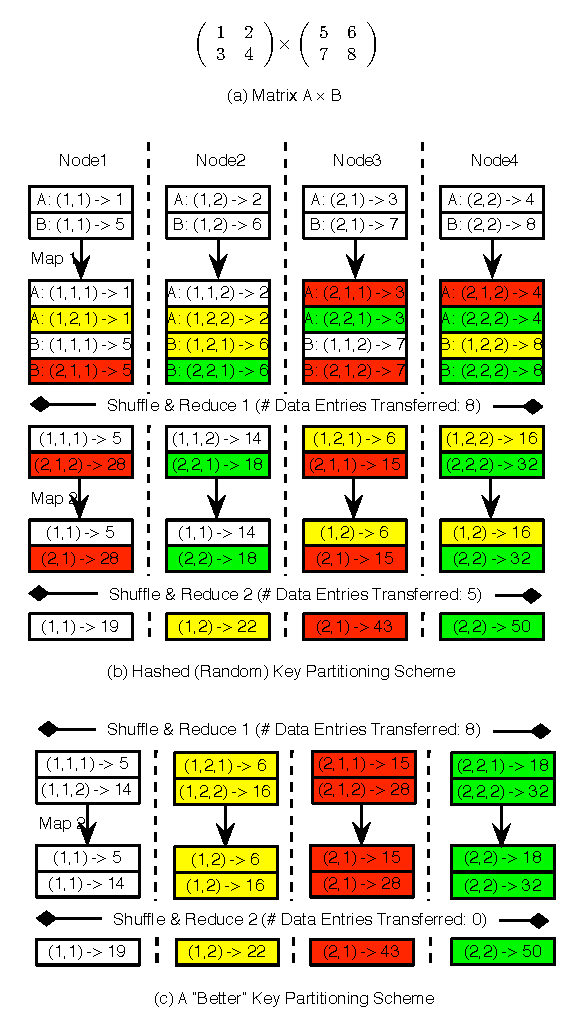
\includegraphics[width=1\columnwidth]{figure1}
\caption{An Example of the MapReduce-style Matrix Multiplication Algorithm with Different Key Partitioning Schemes 
}
\label{fig:matrixExample}
%\vspace{-0.2in}
\end{figure}

We present the Confluence Key Partitioning (CKP) scheme for iterative distributed operations. 
Based on a set of key dependencies, CKP binds key partitions in 
different iterations and reduces the shuffle size to the maximum
extent. 
Most distributed computing paradigms, such as Spark~\cite{zaharia2012resilient} and Twister~\cite{ekanayake2010twister},
provide an interface for adding a user-defined partitioner for shuffle operations.
We implement CKP in Spark and programmers can apply CKP to various 
kinds of distributed applications by add a single line of code
in the program.
% CKP automatically generates an efficient key partitioning 
% scheme from the KDG. 
% This user-defined key partitioning scheme guides the assignment of data entries 
% to their designated nodes. 
We illustrate with analysis and experiment to real-life applications 
to show that by applying the CKP scheme, 
the shuffle size of multiple computing
iterations reduces significantly with a predictable percentage, 
e.g., 100\% shuffle size reduction in an iteration of the MovieLensALS algorithm. 
%in polynomial time,
% Note that CKP will not impact the workload skewness in most cases; 
% that is, the standard deviation of the computing workloads of the
% nodes in the cluster after applying CKP will not be larger than that
% with the random hashing scheme.

To the best of our knowledge, we are the first to 
represent the logic of iterative distributed operations
by key dependency, and the first to reduce the 
shuffle size with a predictable value by considering the key dependency 
across multiple iterations in a key partitioning scheme.
%\textcolor{red}{Performance}
Our major contributions are listed as follows.

\begin{itemize}
% \setlength{\itemsep}{0pt}
% \setlength{\parskip}{0pt}
% \setlength{\parsep}{0pt}
\item \textbf{Precise}: 
We invented the simple yet powerful notion of Confluence key dependency to precisely capture the logic of data transformation in iterative distributed operations. 
We defined the transform-and-shuffle primitive that can generally describe all iterative distributed operations. 

\item \textbf{Efficient}: We presented the Confluence Key Partitioning (CKP) scheme to 
greatly reduce the shuffle size in iterative distributed operations.
% CKP makes use of the model of Confluence key dependency and the technique of binding key partitions to partition data to locations where they will be processed later.
CKP is efficient and does not introduce extra workload skewness. 

\item \textbf{Universal}: We showed that CKP is easily applicable to diverse real-life distributed applications.
We provided a simple interface in distributed paradigms that allows 
programmers to apply CKP with one single line of code.
% , and it greatly reduces the shuffle size.

% \item We invented the new data structure Key Dependency Graph to depict the iterative key dependency
% and used the Confluence Key Partitioning (CKP) scheme to decrease the shuffle traffic
% across distributed computing iterations.

% \item We created the method to analyze the data transfer size and the workload skewness when using CKP, which offers the solid shuffle traffic improvement with guarantees. 

% \item We implemented CKP in Spark and illustrated the use of CKP with typical iterative distributed applications from different fields. 
% The experiment on a medium-size cluster demonstrates that CKP reduces the overall shuffle traffic by as much as 50\%.  
\end{itemize}


The rest of the paper is organized as follows. 
In Section~\ref{section:background}, 
we introduce the model of iterative distributed operations and the 
iterative shuffle size, give the definition of Confluence 
key dependency, and analyze the shuffle size of 
the random key partitioning scheme based on the Confluence key dependency.
We present the Confluence key partitioning scheme in Section~\ref{section:confluence}.
Section~\ref{section:application} introduces the application of CKP
and its limitations, 
and Section~\ref{section:implement} discusses 
implementation details of CKP in distributed paradigms.
Evaluation results of CKP are presented in Section~\ref{section:evaluation}. 
We discuss the related work in Section~\ref{section:relatedWork} and
conclude the paper and suggest the future work in
Section~\ref{section:conclusion}.


\section{Model and Definition}\label{section:background}
\subsection{Iterative Distributed Operations}
Datasets of large volumes cannot be stored in a single computer node
and are often separated into several partitions, 
where each partition is distributed to a node in a computer cluster. 
We refer to a dataset which is separately stored in several nodes as a distributed dataset. 
A function whose input includes a distributed dataset is called a distributed operation.
Each entry of the distributed dataset can be represented as a key-value pair. 
%\textcolor{red}{How to obtain each entry in the dataset. }

% In many distributed paradigms, there are often several
% iterations involving different distributed operations being applied
% to an input dataset before final results are obtained. 
% Each iteration usually takes outputs of the previous iteration as
% the input dataset. 

For iterative distributed
operations, we refer to the general iterative transform-and-shuffle operations. 
In each iteration of the iterative distributed operation, 
the ``transform'' primitive performs one or more transformation operations on 
input datasets in each local node.
The ``shuffle'' primitive would
re-partition the datasets by transferring data entries with
the same keys to a designated location and grouping entries of the same key to a key-value pair, as the input for the next iteration. 
% This value is actually a list of the values that associate with the key.
% and the output of each data entry of the shuffle primitive is also called as the key-value-list pair in this paper.
Each iteration of distributed operation is in the form of a series of transformations plus at most one shuffle operation.

Note that the division of distributed operations by transform-and-shuffle is similar to the paradigm of 
MapReduce~\cite{dean2008mapreduce}, which divides the operation into two primitives: map and reduce.
They are slightly different but can be equivalent in the context of iterative distributed operations.  
The shuffle primitive is equivalent to the shuffle operation of the reduce primitive in MapReduce. 
It does not involve any transformation on data.
While the transform primitive is equivalent to the reduce operation
(excluding the shuffle operation) in the reduce primitive plus the map primitive of the next iteration of a MapReduce operation. 
The shuffle primitive is also called the shuffle operation,
and the transform primitive is called the transform operation or, simply, 
transformation.

% in the matrix multiplication example in Section~\ref{section:introduction} is slightly different from the definition here. 
% The transform primitive of an iteration is equivalent to 
% the reduce operation in the previous iteration without the shuffle operation plus the map operation of the next iteration in MapReduce. 
% The shuffle primitive is only 

% For instance, in the matrix multiplication example in Section~\ref{section:introduction},
% In the example, 
% the reduce primitive aggregate the value list of each key to a value, which follows the traditional style of MapReduce. 
% While by the definition here, the aggregate operations should join other data transformation operation in the map primitive of the next iteration. 

% In the rest of this paper, the terms of the reduce primitive and the shuffle operation may be used interchangeably. 

% One typical example of the distributed operation is
% MapReduce~\cite{dean2008mapreduce}, 
% which divides the operation into two primitives: map and reduce.
Most iterative distributed paradigms such as the in-memory paradigm
Spark~\cite{zaharia2012resilient} and the distributed database query
engine Hive~\cite{thusoo2009hive} can be equated to iterative transform-and-shuffle operations.
The matrix multiplication example in Section~\ref{section:introduction}
follows the traditional MapReduce interpretation. 
From now on in this paper, we use the transform-and-shuffle interpretation when we describe iterative distributed operations.

% The traffic pattern of the data to shuffle in each iteration is directly
% dictated by the key partitioning scheme.
% A random or careless key partitioning scheme may cause unnecessary
% shuffle traffic across multiple iterations of distributed operations.
% This is what we set out to improve using our partitioning scheme.


% \subsection{Dependency Graph}
% The dependency graph is a directed graph usually used for
% describing the dependency relationship of instructions, tasks, data, etc
% \cite{sakellariou2004hybrid,zhao2006scheduling,isard2007dryad}.
% The scheduler can use the dependency graph to decide the order the execution of instructions or tasks. 
% In distributed frameworks, the scheduler uses the data dependency graph
% or task dependency graph to make the tasks execute in parallel in the
% cluster.
% As the tasks are meant to process their specific data, the task dependency
% graph is the data dependency graph as well.

% In the data dependency graph, the datasets are divided into graph nodes
% based on locations and the dependency relationship is
% constructed upon the execution stages and data locations.
% The data partition information is specific to the application running
% situation and the cluster environment.
% In the key dependency graph proposed in this paper, the construction of
% the graph does not use any data partitioning information, but considers
% the key dependency of data, which depends on the
% application logic.



\subsection{Iterative Shuffle Size}\label{section:model}
We model the overall shuffle size of iterative
distributed operations and discuss the time complexity of obtaining
the optimal key partitioning scheme that minimizes the overall shuffle
size. Table~\ref{table:symbol} lists some symbols we use in this paper
for reference. 

For iterative distributed operations, the result of the $i_{th}$ iteration can be obtained recursively by:
\begin{equation*}\label{eq:t}
A'_i=T_i(A_i)
\end{equation*}
\begin{equation*}\label{eq:s}
A_{i+1}=S_i(A'_i)
\end{equation*}
, where $A_i$ is the output of iteration $i-1$ as well as the input of iteration $i$, 
$T_i$ is the transform operation of iteration $i$ that operates on $A_i$ locally without changing the partition locality, 
and $S_i$ is the shuffle operation of iteration $i$ that takes the output $A'_i$ of the transform operation as the input.  
$A_i$ and $A'_i$ define not only key-value pairs of datasets, but also their partition locality. 
The keys of $A'_i$ and $A_{i+1}$ are the same, but their partition localities are different. 
In the first iteration, when $i$ equals 1, 
$A_1$ represents the raw input datasets before any processing.  

Suppose in the shuffle operation of iteration $i$, in order to shuffle transformation outputs of an entry $a \in A_i$ to its partition location, 
the shuffle size is a function of $a$ and $A_{i+1}$: $g_i(a,A_{i+1})$. 
The returned value of function $g_i$ can be different in different key partitioning schemes for $A_{i+1}$. 
The shuffle size of iteration $i$ is: 
\begin{equation*}\label{eq:gi}
\begin{aligned}
G_i=\sum_{a \in A_i} g_i(a,A_{i+1}).
\end{aligned}
\end{equation*}

% Within the same $i_{th}$ iteration, for $\forall a_p, a_q \in A_i$ where $a_p \neq a_q$, values of $g_i(a_p,A_{i+1})$ and $g_i(a_q,A_{i+1})$ are independent of each other in terms of $a$. 
% If the value of $g_i(a_p,A_{i+1})$ changes due to a different partition location of $A_{i+1}$, the value of $g_i(a_q,A_{i+1})$ remains unchanged unless $a_q$ is also partitioned to a different location. 

If $m$ iterations are required to compute the final result, 
the overall accumulated shuffle size for obtaining the final result is
\begin{equation}\label{eq:g}
G=\sum_{i=1}^{m} G_i=\sum_{i=1}^{m} \sum_{a \in A_i} g_i(a,A_{i+1}).
\end{equation}


% \red{If values of $G_i (1 \leq i \leq m)$ are independent of each other, 
% $G$ is a linear function and $G$ can be minimized simply by minimizing each $g_i(a,A_{i+1})$. Not correct now because they are not independent}
% However, most usually, $G_i$ and $G_{i+1}$ are correlated.
% The value of $G_i$ depends on the logic of the transform function $T_i$ in Formula~(\ref{eq:t}), 
% and the partition locality of datasets $ A_{i}$ and $A_{i+1}$. 
% The partition locality of $A_{i+1}$
% will again affect the value of $G_{i+1}$.
%\textcolor{red}{add Markov-Chain-like relation here}

If contents (including key-value pairs and the partition locality) of $A_i (i=1,2,...,m)$ are already known, to find out the optimal key partitioning scheme that minimizes 
%A clumsy and straightforward way to minimize 
the overall shuffle size $G$,  %is 
we need to exhaustively explore the possible key partition of all the key-value pairs in $A_{i+1}$ across all the iterations. 
By calculating the overall shuffle size of each scheme, the optimal solution is the scheme with the minimal size. 
The time complexity of the exhaustive method is $O(n^{\sum_{i=1}^{m+1} |A_i|}$), 
where $n$ is the number of nodes in the cluster and $|A_i|$ is the number of data entries of $A_i$, 
which indicates it is a complex problem. 

In fact, we usually do not know the contents of $A_i$ and cannot explore the data partition
for the next iteration until the program has actually finished the $i_{th}$ iteration. 
Considering this limitation and the time complexity, the idea of finding out the optimal partition schemes for all the iterations to minimize the overall data transfer size $G$ is infeasible. 
% In the rest of this paper, the shuffle size is used to refer to the data transfer size of the shuffle operation. 

\begin{table}[!t]
% increase table row spacing, adjust to taste
\renewcommand{\arraystretch}{1}
% \extrarowheight as needed to properly center the text within the cells
\caption{Symbol Reference}\label{table:symbol}
\centering
% Some packages, such as MDW tools, offer better commands for making tables
% than the plain LaTeX2e tabular which is used here.
%\begin{tabular}{|c||c|c|}
\begin{tabularx}{0.49\textwidth}{ c | c }
\hline
\textbf{Symbol} & \textbf{Description}  \\
\hline
$A_i$ & Input dataset for iteration $i$\\
\hline
$A'_i$  & Transformation Output in iteration $i$   \\
\hline
$D_k$ & Set of input entries of the transform operation \\
&(in the specified iteration) that have key $k$\\
\hline
$D'_k$ & Outputs of the transform operation with $D_k$ as the input\\
\hline
\end{tabularx}
%\end{tabular}
\end{table}

\subsection{Confluence Key Dependency}\label{section:dependency}
We define the Confluence key dependency, or for convenience, 
simply called key dependency in the rest of this paper,
to represent transformation logic in every iteration
of a distributed operation. 
Given a key-value pair as the input to an iteration of a distributed operation,
the transform operation will generate a (or a set of) new key-value pair(s) based on its logic. 


Formally, for a set of input key-value pairs and output key-value pairs 
in an iteration of a distributed operation, 
we define their key dependency as 
\begin{equation}\label{eq:dependency}
k \Rightarrow_{pr} f(k)
\end{equation}
, where $k$ is a key, 
$f$ is a mapping function of $k$, 
and $f(k)$ is another key. 
For now, we do not care about what $f$ is like, and consider $f(k)$
as an arbitrary key. 
The symbol ``$\Rightarrow_{pr}$'' indicates the fact that 
for any data entry whose key is $k$, after the transform primitive, 
the probability of that the key of an output data entry is $f(k)$ is $pr$.
By definition, we have:
\begin{equation*}\label{eq:dependencyDefine}
\begin{aligned}
k_0 \Rightarrow_{pr} f(k_0) \equiv 
& \forall \langle k,v \rangle \in \{ \langle k,v \rangle | k = k_0\}: \\
& p(k_{t( \langle k,v \rangle)} = f(k)) = pr
\end{aligned}
\end{equation*}
, where $t(\langle k,v \rangle)$ is the transform operation on $\langle k,v \rangle$ and outputs 
a set of key-value pairs, $k_d$ is one of the keys in dataset $d$,
and $p$ is the probability function. 

In the key dependency, we call $k$ the input key, $f(k)$ the mapped key, 
and $pr$ the dependency probability.
This key dependency can be read and grasped as 
"input key $k$ has a chance of $pr$ to map to mapped key f(k)" after transformation in the corresponding iteration. 

A programmer is supposed to be well acquainted with the logic of the transform operation $t$. 
By saying that we know the key dependency for a specific iterative distributed operation,
it means that we are able to calculate $pr$ by the probability function 
$p$ for specific $k$ and $f(k)$.
In the matrix multiplication example, we can easily deduce
the key dependency of the second iteration: 
$\forall i, j, p \in domain: (i, j, p) \Rightarrow_{1.0} (i, j)$.  
Specially, the key mapping function is $f((i, j, p)) = (i, j)$.
% it means that we know what the output key-value pairs will be 
% for an input key-value pair in every computing iteration. 

% We use the key dependency graph (introduced later) to portrait the iterative key dependency
% so that it is comprehensible to the computer. 
% Every distributed operation has its own key dependency
% and it relies on the programmer to understand the iterative key dependency based on the application logic
% and construct the key dependency graph.

\subsection{Random Key Partitioning}\label{section:rkp}
We will show that the random key partitioning scheme (RKP) generates no less shuffle size than almost any other key partitioning schemes. 
In RKP, a key is assigned a random partition location in the shuffle operation. 
RKP is widely used in popular distributed paradigms.
For example, Spark~\cite{zaharia2012resilient} uses the hash-based key partitioning scheme, which partitions keys based on their hash values. 

As mentioned in in Section~\ref{section:model}, the shuffle size $g_i(a, A_{i+1})$ to shuffle transformation outputs of entry $a$ is different in different key partitioning schemes. 
Given a key dependency implicated by a distributed operation, we discuss how to calculate $g_i(a, A_{i+1})$ in a specific key partitioning scheme. 
We set off from RKP.


In a cluster of $n$ nodes, using RKP, the probability of a transformed key-value pair 
is assigned and partitioned to another node (which indicates a network transfer) is $(n-1)/n$.

In iteration i, let $D_{k}$ denote all transform operation inputs that have key $k$, $D'_{k}$
denote transform operation outputs after transforming $D_{k}$, 
and $|D|$ and $|D'|$ denote the volume of dataset $D$ and $D'$. 
% In the rest of the discussion, we think of the size of every key-value pair in a dataset is the same. 
% % Considering the difference between the sizes of different key-value pairs
% % in $D$ will work, but it will greatly complicated our discussion. 
% Therefore, $|D|$ equals the size 
% of each key-value pair times the number of key-value pairs in $D$.
Given a set of key dependencies $k \Rightarrow_{pr_j} k_j, \sum_j pr_j = 1$, 
the expected shuffle size to transfer $D'_k$ in RKP is:
\begin{equation}\label{eq:rkp_gi}
\begin{aligned}
\sum_{a \in D_k} g_i(a, A_{i+1}) = \sum_j \frac{n-1}{n} pr_j  |D'_{k}| 
&= \frac{n-1}{n} |D'_{k}|\\
&\approx |D'_{k}|.
\end{aligned}
\end{equation}

In cases that $n$ is big in a large cluster, the approximately equal sign
in Formula~\ref{eq:rkp_gi} can be thought of as an equal sign. 
Note that the key dependency does not affect the shuffle size of an iteration in RKP at all. 
For any key partitioning scheme, the shuffle size cannot be larger than 
the volume of the shuffle operation. 
That is, $\sum_{a \in D_k} g_i(a, A_{i+1}) \leq |D'_k|$ for any key partitioning scheme.
By summing up the shuffle sizes for all keys in all iterations by Formula~\ref{eq:g},
we can easily conclude that
the overall shuffle size of RKP is no less than almost any other key partitioning scheme. 

% Suppose that $a'$ is the set of input data entries that have the same key as $a$ right before the shuffle operation and $p_j$ denotes the percentage of data entries of $a'$ that lie in Node $j$, where $\sum_{j=1}^{n} p_i=1$.
% We have
% \begin{equation}\label{eq:si2}
% s_i(a,A'_i)= \sum_{j=1}^{n} [\frac{1}{n}|a|(1-p_j)]=\frac{(n-1)} {n}\cdot |a|
% \end{equation}
% , where $|a|$ is the length of the value list of $a$, which is also the number of data entries in $a'$. 
% It shows that if $a$ is randomly partitioned to a node, 
% the distribution of $a'$ does not affect the data transfer size for collecting $a$. 

\section{Confluence}\label{section:confluence}
Although it is hard to find the optimal partition solution to minimize the overall shuffle size,
we discover that 
if the transformation logic of a specific distributed operation is already known, 
the shuffle size can be reduced to the maximum extent %in polynomial time 
by exploring the key dependency of different iterations. 

The key dependency is to represent the logic of transform operations, 
while the key partitioning scheme is to indicate the logic of shuffle operations. 
By the observation that the RKP shuffle size can be deduced from the key dependency, we have the intuition that we can
use the key dependency to discover other key partitioning schemes that produce a smaller shuffle size. 

In this section, we present the Confluence key partitioning scheme
that makes use of the key dependency to reduce the shuffle size by binding 
key partition locations. 
We also analyze that the Confluence Key Partitioning scheme does not 
increase the workload skewness.

% This section firstly describes the construction process of the key dependency graphs, as well as its properties. 
% After that, we present Confluence Key Partitioning Scheme, which decreases the overall iterative shuffle size by applying the properties of the key dependency graph, while not increasing the workload skewness. 

\subsection{Key Partition Binding}\label{section:binding}
We will show that binding partitions of input keys to mapped keys based on the key dependency reduces the shuffle size.
Assume that we have a set of key 
dependencies $k \Rightarrow_{pr_j} k_j, \sum_{j} pr_j = 1$ in an arbitrary iteration $i$. 
Now suppose that a key partitioning scheme $X$ has always partitioned
shuffle output data that have key $k$ in the previous iteration $i-1$ to the same computer node where 
shuffle output data that have key $k_x$ in this iteration $i$ will be partitioned. 
We say that key partitioning scheme $X$ binds the partition of 
input key $k$ to mapped key $k_x$ in this iteration $i$. 
% For shuffle outputs that have other keys, scheme $X$ partitions them by the hash values of their keys. 

By the definition of the key dependency and recalling that 
the shuffle size only refers to cross-node data traffic,
we easily deduct the following theorem.
\newtheorem*{theorem*}{\textbf{Binding Theorem}}
\begin{theorem*}\label{thm:binding}
Suppose a key dependency $k \Rightarrow_{pr} f(k)$ in an iteration of a distributed operation,
if the partition of key $k$ was bound to $f(k)$ in this iteration, 
the shuffle size for transferring transformation output data that have key $f(k)$ after transforming $D_k$ is zero in this iteration.
\end{theorem*}

The insight of the binding theorem is that if we know the key dependency 
for a dataset in an specific iteration,  we can prepare the partition
of the dataset in the previous iteration by the notion of binding keys so that the dataset
will do local shuffling in this iteration and it will incur no cross-node traffic. 

In such a scheme X, reusing the symbols in Section~\ref{section:rkp}, 
by the binding theorem, the expected shuffle size to transfer 
transformation outputs of the $D_k$ is: $\sum_{a \in D_k} g_i(a, A_{i+1}) = \frac{n-1}{n} (1 - pr_x) |D'_{k}|$.
The shuffle size reduction of scheme X compared to scheme RKP is 
$ \Delta \approx pr_x |D'_{k}|$. 
The value of $|D'_{k}|$ is a constant for a given transform operation and input $D_k$. 
The larger $pr_x$ is, the greater scheme X reduces the shuffle size than RKP does. 

There are two constraints when binding key partitions. 
First, key partition binding can often be used in all but the first iteration of a distributed operation.
The reason is that most distributed frameworks do not support specifying the partition locations of input data loaded from a file system, which means 
binding key partitions in the first iteration is not feasible. 
But it could be used in the following iterations.

The second constraint is that for a single copy of dataset, any input key can be bound to at most one mapped 
key, because a key should have a unique partition. 
This constraint indicates for all key dependencies with the same input key, only one can be selected for key partition binding in an iteration. 
These two constraints are considered as common sense when we design new key partitioning schemes.

\begin{figure}[!t]
\removelatexerror

\begin{algorithm}[H]
  In a specific iteration $i$,
  \ForEach{key $k$}{
    \tcc{$K$ is a key dependency set}
    $K$ = $\{ k \Rightarrow_{pr_j} f_j(k) | j = 1, 2, ..., \sum_j pr_j \leq 1 \}$ ; \\
    Find $J$ such that $\forall j, pr_j \leq pr_{J}$; \\
    Bind input key $k$ to mapped key $f_J(k)$;
}

\caption{Enhanced Key Partitioning Scheme X}
\label{algo:x}
\end{algorithm}
\end{figure}


\subsection{Confluence Key Partitioning}\label{section:ckp}
Surprisingly, by the binding theorem, we find that
binding key dependency always reduces shuffle size as compared to RKP. 
Note that by binding key partitions, the shuffle size reduction is 
linearly proportional to the dependency probability. 
We can further enhance scheme X 
by applying key binding based on the key dependency with the 
maximum dependency probability for each key in an specific iteration (Algorithm~\ref{algo:x}). 

A problem exists in the enhanced scheme X. 
The key dependency is usually provided by programmers.
In just one iteration, programmers need find a distinguished
key dependency set for every input key. 
The key dependency sets of different input keys can be different. 
The time complexity of finding the key dependency in an iteration is the size of a key dependency set (usually small and can be considered as a constant) 
times the number of keys (usually large), 
or roughly, $O$(\# of keys), which is usually large. 


We presents the efficient Confluence Key Partitioning (CKP) scheme that 
reduces or even eliminates 
the shuffle size in each iteration with as little as $O(1)$ time complexity. 
The procedure of applying CKP is shown in Algorithm~\ref{algo:CKP}.
In an iteration, instead of finding a distinguished key dependency set for 
every input key, CKP finds one general key dependency set that is applicable 
to any input key. 

For example, in the second iteration of matrix multiplication, 
instead of finding key dependency $(1, 0, 0) \Rightarrow_{1} (1, 0)$ 
for input key $(1,0,0)$ and $(1,0,1) \Rightarrow_{1} (1,0)$ 
for input key $(1,0,1)$, respectively, 
we can define $(1, 0, p) \Rightarrow_{1} (1,0)$ for any $p$ in general. 
Or more generally, we can define $(i, j, p) \Rightarrow_{1} (i, j)$ 
generally for any $i, j, p$. 

A feature of CKP is that it allows a programmer to decide whether a specific iteration should apply key partition binding or not. 
In some iterations, it may happen that programmers fail to find the key dependency, 
or the maximum dependency probability of the key dependency set is very small, 
and thus applying CKP is trivial. 
In these cases, CKP let programmers decide not to bind key partitions. 
Further discussion about these cases will be presented in Section~\ref{section:limitation}.
When a key dependency with a large dependency probability exists in an iteration, key partition binding can be applied to reduce shuffle size.

A question about the CKP algorithm is how programmers figure out the key dependency set in an iteration. 
The key dependency is  derived from the transform operation logic. 
% For input entries with a specific key, the transform operation outputs 
% a set of new entries. 
In some cases, for input key-value entries with a specific key, 
the transform operation always generates output entries with predictable keys, 
regardless what the values are. 
The matrix multiplication algorithm falls in this case. 
Finding key dependency such cases is usually simple, 
and a programmer may start from the domain of the input keys and 
derive the general key dependency for each range of the domain.
In some other cases, keys of the output entries are also affected by 
the values of the input key-value entries. 
In these cases, a programmer need also consider the key-value entries as 
a whole to deduct what mapped keys will be and what probability it is
to generate an output entry with each mapped key.
We will discuss more about finding the key dependency with real-life examples in Section~\ref{section:application}.

There is an implicit in the CKP algorithm. 
For iterations that do not apply key partition binding, 
the input keys are randomly partitioned, just as in RKP.

CKP reduces the shuffle size in all iterations that apply key partition binding.
The shuffle size reduction in each binding iteration compared to RKP is $ \Delta \approx \sum_k pr_J |D'_k|$ (recalling the shuffle size reduction by 
key partition binding in Section~\ref{section:binding}). 
For other iterations that do not applied key partition binding, 
the CKP shuffle size is the same as that of RKP.
In all, CKP reduces the shuffle size by a percentage of $pr_J$ in each 
iteration that applies key partition binding. 
When $pr_J$ equals 1 in an iteration, the shuffle size is 0 in that iteration.

\begin{figure}[!t]
\removelatexerror

\begin{algorithm}[H]
\ForEach{iteration $i$}{
  \tcc{Programmers decide that}
  $b$ = Should iteration $i$ apply key partition binding? \\
  \If{$b = True$}{
    \tcc{$K$ is a key dependency set}
    Find $\forall k, K =$ 
    $\{ k \Rightarrow_{pr_j} f_j(k) | j = 1, 2, ..., \sum_j pr_j \leq 1 \}$ ; \\
    Find $J$ such that $\forall j, pr_j \leq pr_{J}$; \\
    $\forall k$, bind input key $k$ to mapped key $f_J(k)$;
  }
}

\caption{Confluence Key Partitioning}
\label{algo:CKP}
\end{algorithm}
\end{figure}



\subsection{Workload Skewness Analysis}\label{section:skew}
CKP does not increase the workload skewness in most applications. 
The workload of a node is the number of input entries for the transform
operation in that node and 
the workload skewness of an iteration is the standard deviation of the workloads of different nodes in that iteration. 
% The math symbols in Section~\ref{section:CKP} are reused here without duplicated definition. 
% Only the data entries that associate with the pure confluence subgraphs are counted as the other data (if any) are randomly partitioned in both RKP and 
% CKP and will not affect the standard deviation of the workloads.


We compare workload skewness of CKP and RKP in iterations 
that apply key partition binding.
In unbound iterations, the key partitioning policy of CKP is the same as that of RKP, and the workload skewness in these iterations is the same in both schemes.
Suppose in one of such iterations, keys of input entries follow a distribution $Dist$. 
In RKP, these input keys have been uniformly partitioned, 
and the workload skewness is the standard deviation of $Dist$ times 
% the total number of input entries times
the average number of distinguished input keys in each node. 

In CKP, in a binding iteration, suppose two conditions: 
1) input keys are uniformly bound to mapped keys;
2) the mapped keys, which is also the input keys of the next iteration, will be uniformly partitioned in the shuffle operation.
The first condition means that the expected number of distinguished input keys bound to every mapped key is the same.
If both conditions are satisfied, it indicates that the input keys have also 
been uniformly partitioned in the previous iteration,
and therefore, the workload skewness is the same as that of RKP.
The second condition will be eventually satisfied, as the last iteration always randomly partitions keys. 
If the first condition is always true in all iterations, 
the second condition can be proved to be always true by induction from the last iteration back to previous iterations. 

In all, if input keys are uniformly bound to mapped keys in all iterations, the workload skewness of CKP 
is the same as that of RKP. 
Luckily, this condition is true in most applications we observe.
For example, in the second iteration of matrix multiplication, 
the number of input keys $(i,j,p)$ that
are bound to mapped key $(i,j)$ is the dimension size of the matrix.
In the MovieLensALS algorithm introduced later in Section~\ref{section:application}, the expected number of input keys $(userId, itemId)$
that are bound to mapped key $userId$ is the average number of items all users have bought.
In a few cases (e.g., KMeans in Section~\ref{section:application}) when this condition does not hold, 
we find that the workload skewness difference of CKP and RKP is so small  that it could be ignored, regarding the shuffle size CKP reduces.

% In all iterations when RKP is applied, every entry is a uniformly-partitioned entry, the expected workloads of the all the nodes are the same and the expected workload skewness is 0. 

% When CKP is applied, as each output entry of the shuffle operation is the uniformly-partitioned entry in Iteration $u$, the workloads of all the nodes are the same in Iteration $u+1$. 
% Therefore, $L_{u+1}=0$.

% In Iterations from $u+2$ to $w+1$, 
% it can be divided into two phases based on the logic of the distributed operations. 
% Suppose that Iteration $u' (u+1 \leq u' \leq w)$ is such an iteration that in every iteration from $u+1$ to $u'-1$, each input entry of the map primitive is expected to generate the same number of output entries of the shuffle operation, and in Iteration $u'$, the expected number of output entries of the shuffle operation generated by each map input entry is unknown or not the same. 
% Note that such Iteration $u'$ may not exist and in this case, we denote it as $u'=w+1$. 

% \textbf{Phase 1}: From Iteration $u+2$ to $u'$, 
% the workloads are the same in all the nodes and the workload skewness of every iteration is 0.

% \textbf{Phase 2}: From Iteration $u'+1$ to $w+1$, 
% the workloads of the nodes in each iteration are unpredictable, 
% which are dependent on the number of data entries that can be generated by the data localized in each node. Therefore, $L_i \geq 0, u'+1 \leq i \leq w+1$.

% Although the workload skewness of CKP in Phase 2 is unpredictable,
% fortunately, such Iteration $u'$ does not exist in many distributed operation, 
% including matrix multiplication and the other distributed applications (MovieLensALS, MultiAdjacentList and KMeans) introduced in Section~\ref{section:application}. 
% In these applications, the expected workload skewness of CKP is 0, which is the same as that of RKP.
% In the distributed application where $u'$ does exist, the workload skewness may not be 0 and specific workload skew analysis is needed for this specific application.


\subsection{Affect of Inaccurate Key Dependency}\label{section:inaccurate}
Note that programmers do not need to change the original logic of applications in order to apply CKP. 
Applying any key partition scheme, including CKP, will not affect
the logic correctness of the applications, but only affect the traffic 
performance of shuffle (shuffle size and workload skewness). 

An inaccurate key dependency means a key dependency with 
an inaccurate dependency probability. 
A dependency probability of a key dependency implies 
how much CKP reduces the shuffle size compared to RKP.
When an inaccurate key dependency is applied
in CKP, the shuffle size reduction
is related to the actual dependency probability, not to the inaccurate one. 
At all events, the shuffle size of CKP is no greater than that of RKP. 

As to the workload skewness, the inaccurate key dependency may lead to 
a different key partition binding and unpredictable workload skewness may exist. 
But as CKP randomly partitions mapped keys in every iteration whose next iteration does not apply key partition binding, 
the workload skewness readjusts to the same as RKP then.



\section{Application}\label{section:application}
% In this section, we illustrate how CKP can be applied to the matrix multiplication algorithm straightforwardly. 
In this section, we show how CKP is applied in various
iterative distributed applications, by digging out the key dependency 
with a large dependency probability
in some iterations. 
We also discuss limitations of CKP when in some circumstances it is not applicable, and solutions to handle these limitations. 

We find that many applications have key dependency with 
a large dependency probability in some iteration(s).
For example, 
in the second iteration of the matrix multiplication algorithm, 
the transform operation does a many-to-one processing and the key dependency is obvious, 
$\forall$ key $(i,j,p)$, $(i,j,p) \Rightarrow_{1} (i,j)$,
which has 100\% dependency probability for all key dependencies.
In some applications, the dependency probability is not 100\% but 
is still large enough to apply CKP.
We illustrate the techniques of finding the key dependency of iterative
distributed operations with the real-life application examples from 
different fields.
A summary of the CKP shuffle size improvements to the distributed applications discussed below is shown in Table~\ref{table:reduction}.

\begin{table}[!t]
\begin{threeparttable}[b]
% increase table row spacing, adjust to taste
\renewcommand{\arraystretch}{1}
% \extrarowheight as needed to properly center the text within the cells
\caption{CKP Shuffle Size Reduction in Different Distributed Operations}\label{table:reduction}
\centering
% Some packages, such as MDW tools, offer better commands for making tables
% than the plain LaTeX2e tabular which is used here.
%\begin{tabular}{|c||c|c|}
\begin{tabularx}{0.5\textwidth}{ c || c }
\hline
\textbf{Distributed Operations} & \textbf{CKP Shuffle Size Reduction}  \\
\hline
MatrixMultiplication & $n^3 for R^{n \times n}$\\
\hline
MovieLensALS  & \# of $(user,item)$ entries  \\%; input file size 640 MB 
\hline
GoogleAlbum & \# of album entries and user entries \\
\hline
PageRank & volume of link lists of all URL's \\
& in every join iteration\\
\hline
MultiAdjacentList  & 1/2 the RKP shuffle size in every iteration \\
\hline
KMeans & $|A| \cdot \sum_{i=j+1}^{m} p_{ij}$ \tnote{1} \\
& upper bound: $(m-j) |A|$ \\
& lower bound: $0$\\
\hline
\end{tabularx}
\begin{tablenotes}
    \item[1] $|A|$ is the volume of points, $m$ is the number of iterations. 
  \end{tablenotes}
%\end{tabular}
\end{threeparttable}
\end{table}

\begin{figure*}[!t]
\centering
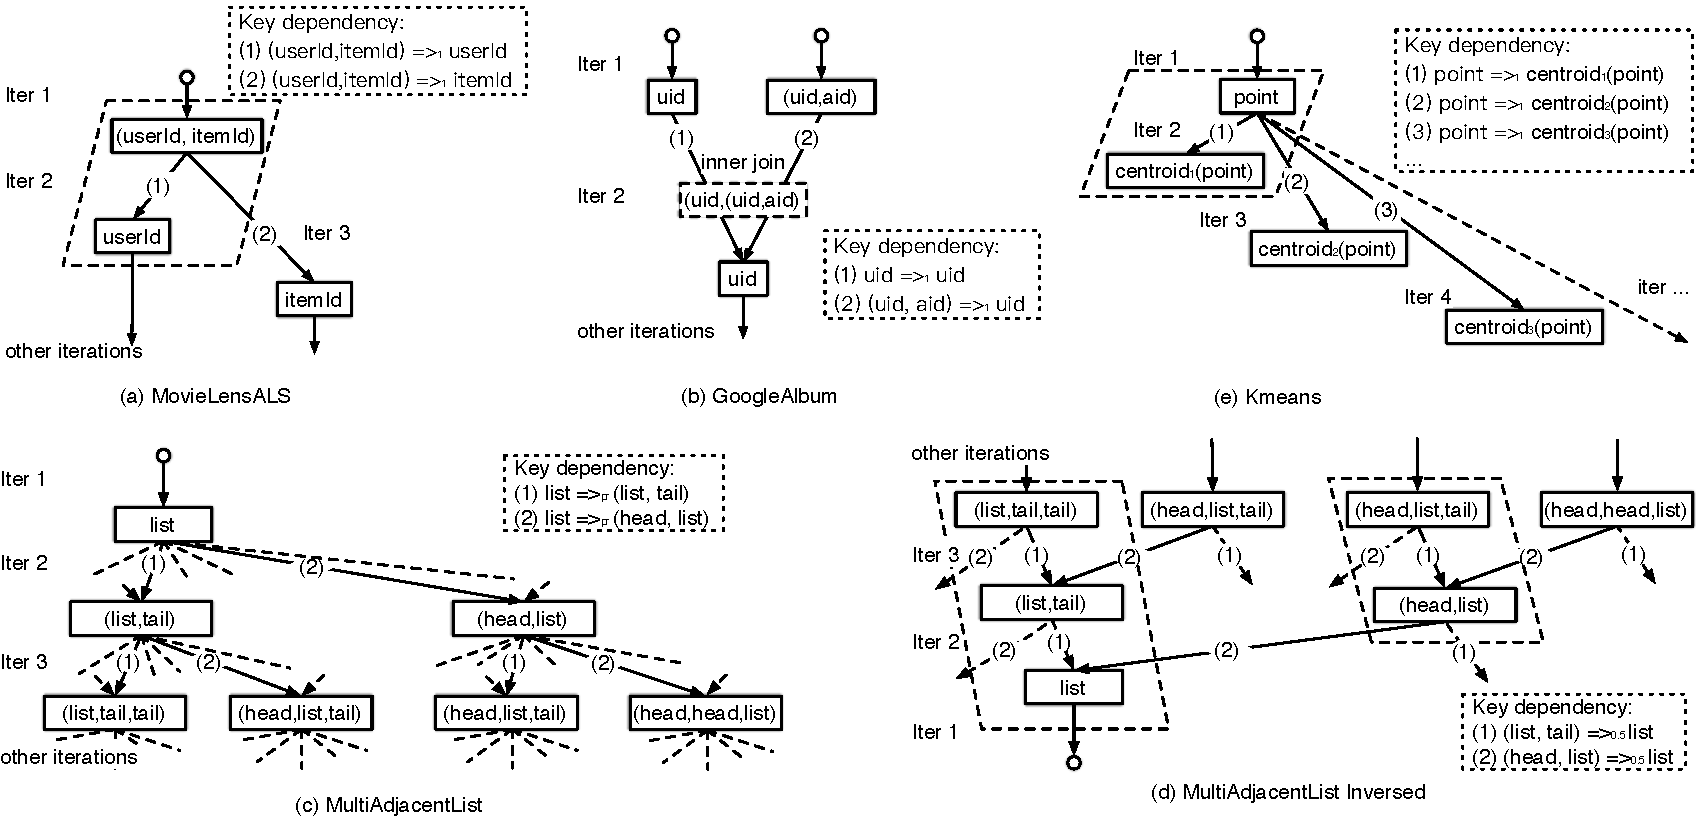
\includegraphics[width=2\columnwidth]{figure4}
\caption{The Transformation Lineage of Keys between Iterations 
and the Key Dependency of Different Applications. Key Partition Binding is Applied to Keys in Iterations Wrapped in Dashed Rhombus Boxes
}
\label{fig:application}
%\vspace{-0.2in}
\end{figure*}


\subsection{MovieLensALS}
MovieLensALS \cite{movielensals} is a
recommendation application that uses the Alternating Least Squares (ALS)
method in collaborative filtering in order to recommend product
items to users based on the user-item rating information.
During the execution, it organizes the rating data into user-item
blocks grouped by key ``$(userId, itemId)$".
In the successive iterations, it needs to reorganize the user-item block
data by generating user blocks and item blocks grouped by
key ``$userId$'' and key ``$itemId$'', respectively.
This operation is done in two iterations as shown in Fig.~\ref{fig:application}(a). 

Key dependencies from input key $(userId, ItemId)$ exist in
iteration 2 and iteration 3, respectively.
As these two iterations use the same copy of input dataset, 
by the second constraint of key partition binding, 
we can apply key partition binding in either iteration, 
but not in both.
If we select key dependency $(userId, itemId) \Rightarrow_1
userId$ in iteration 2, the shuffle size generating the user block 
in iteration 2 is $0$, 
and the shuffle size generating the item block in iteration 3 
is the same as that of RKP.


\subsection{GoogleAlbum and PageRank}
CKP can usually be applied to \emph{join} operations in distributed databases.
For example, in a Google album application~\cite{google2012spanner}, 
an entry in table Users is identified by primary key ``$uid$''
and an entry in table Albums by ``$(uid, aid)$'' (Fig.~\ref{fig:application}(b)). 
When an \emph{inner join} operation interleaves these two tables and gets albums for 
each user, the transform operation processes interleaved data 
with key ``$(uid, (uid, aid))$'' to album data with key $uid$. 
The key dependency here is $(uid, (uid, aid)) \Rightarrow_{1} uid$.
In CKP, when binding the interleaved key $(uid, (uid, aid))$ to key $uid$, 
it meaning both binding key $uid$ in table Users to key $uid$ (which is a trivial binding)
and binding key $(uid, aid)$ in table Albums to key $uid$. 

We can also interpret this binding as putting album entries 
of the same user together
in the same node before such an ``inner join'' operation.
Spanner~\cite{google2012spanner} uses the similar notion of 
hierarchical schema to maintain data locality in the distributed database. 
The hierarchical schema specifies data locations once when persisting data in storage, 
while CKP specifies data locations iteratively during the computing procedure of a distributed operation.

Similarly in the famous PageRank algorithm, 
the link list of a URL is represented as $\langle url, links \rangle$,
and the rank of a URL is $\langle url, rank \rangle$, 
where $url$ is the key for both datasets. 
These two datasets are joined to entries in form of 
$\langle url, (links, rank) \rangle$ in multiple iterations (Fig.~\ref{fig:application}(c)).
The key dependency is $url \Rightarrow_{1} url$ for both datasets.
Note that the link list dataset is loaded from a distributed 
file system initially and it has not been partitioned 
by its key $url$. 
Without CKP, entries with key $url_0$ in the link list dataset need
to be transfered to the partition of key $url_0$ in every $join$ iteration.
In CKP, by binding partition of input key $url$ to mapped key $url$, 
the link list dataset is partitioned by its key $url$ first.
Therefore, the link list and the rank with the same URL 
are on the same node in every iteration, 
and no shuffle network traffic incurs in these $join$ operations. 
This partition optimization is also suggested in the usage 
of RDD~\cite{zaharia2012resilient}, 
we formalize it here by the concept of key dependency.
% Though binding partitions of input key $url$ to mapped key $url$ 
% seems trivial, as the link list dataset is loaded from a distributed 
% file system initially and it has not been partitioned 
% by it key $url$, we must apply this key partition binding by 
% partitioning the link list dataset by it key $url$ first.


\subsection{MultiAdjacentList}
MultiAdjacentList~\cite{multiAdjList} is
a graph computing application which generates 
lists of different lengths in a graph by concatenating adjacent nodes 
to the head and the tail of a list, recursively.
In every iteration, for a data entry $\langle L_i, value \rangle$,
key $L_i$ represents a list of length $i$ and 
the value is a set of adjacent nodes to the head or the tail of the list.
The transform operation
generates a group of new lists of length $i+1$ by appending head
nodes and tail nodes to each list. Each new list acts as the new key, and
its new head nodes and tail nodes as the new value.
The iterative transformation of keys in MultiAdjacentList is shown in Fig.~\ref{fig:application}(d).

For any input key $L_i$ in iteration $i$, key dependencies 
are $L_i \Rightarrow_{pr_{j}} (head_{j}, L_i)$ and 
$L_i \Rightarrow_{pr_{l}} (L_i, tail_{l})$ for many different 
$j$'s and $l$'s, because a list $L_i$ may have many adjacent head
or tail nodes. Therefore, values of $pr_{j1}$ and $pr_{j2}$ can be 
small and benefits of applying CKP based on these 
key dependencies is little.
But if we inverse the direction of the key flow as 
in Fig.~\ref{fig:application}(e), we have new key dependencies with 
dependency probability of 0.5. 
The key dependencies of the inversed key flow 
reflects the fact that
an entry with key $(L_i, tail)$ is 50\% generated from entries with 
key $L_i$ (and another 50\% from entries with key $(L_{i-1}, tail)$
, where $L_{i-1}$ is a sublist of $L_i$ cutting off the head node).

% We could select either key dependency to apply CKP to all data
% in every iteration. 
% We cannot use CKP to localize the keys $(heads, L_i)$ and $(L_i, tails)$ with $L_i$, 
% as the datasets corresponding to Key $(heads, L_i)$ and Key $(L'_i, tails)$ may overlap for different $L_i$ and $L'_i$.
% However, the programmer can divide the iterative operations into several smaller iterative operations by dividing the dataset as in Fig.~\ref{fig:alsDivision}(d). 
% In the iterative operations in the dashed boxes, the pure confluence subgraphs exist 
% in their KDG's by the key dependency $L_i \Rightarrow (L_i, tails)$.
% \red{
% Applying CKP to these operations and leaving the other iterative operations
% that are related to the keys $(heads, L_i)$ to be randomly partitioned,
% only half of the datasets need to be shuffled. 
% In the setting that every node has $l$ heads and $l$ tails on average, every map input entry is expected to generate $2 \cdot l$ shuffle output entries in each iteration. Therefore, by the discussion in Section~\ref{section:skew}, the workload skewness of each iteration is 0 when CKP is applied. 
% }

\subsection{KMeans}
KMeans~\cite{kmeans} is a famous clustering algorithm in data mining.
It groups vector points into $k$ clusters where each vector point belongs to the cluster with the minimum mean value. 
This procedure is done in a dedicated number of iterations. 
With the initial $k$ chosen points regarded as centroids of the clusters, 
in each iteration, every point is compared with the $k$ centroids and is grouped into a cluster where the Euclidean distance between the point and the centroid is the smallest. 
After all points are grouped, each new cluster centroid is chosen in the next iteration by the mean of the points in that cluster. 
To calculate the mean of each cluster whose points are located in different nodes, the shuffle operation takes place to partition points of the same cluster to one node. 
A point is always transfromed to an entry with its cluster centroid as the key in every iteration. 

% If the points are bound to the same cluster in every iteration, 
% by using the key dependency $points \Rightarrow centers$ 
% and localizing the points in the same cluster at the first iteration, 
% CKP can eliminate the shuffle size in the successive iterations. 
% However, the affiliation of point to clusters are not stable between iterations. 
% One point that is grouped into one cluster in a iteration can be grouped into another cluster in the next iteration. 
% We estimate the shuffle size in this case. 

Key dependency exists in each cluster iteration of the KMeans algorithm (Fig.~\ref{fig:application}(f)).
% We can observe the key dependency: 
% $\forall i > j, \forall p_i: p_i \Rightarrow_{pr_{ij}} centroid_j(p_i)$.
In CKP, we choose a specific iteration $j$, and bind key partitions of 
the points based on the key dependency $point \Rightarrow_1 centroid_j(point)$.
% We can bind key partitions based on this key dependency 
% in each iteration starting from iteration $j+1$. 
As all iterations use the same copy of the point dataset,
the binding can be interpreted as: if a point is partitioned to a cluster 
in an iteration $j$, 
we bind its partition to this cluster afterwards,
regardless of which cluster it will be actually grouped into in the following iterations.

We can predicate the shuffle size after applying CKP.
Suppose in iteration $i, i > j$, 
$pr_{ij}$ is the probability of that any point is grouped 
into the same cluster as it was grouped into in a previous iteration $j$.
% , where the cluster is denoted as $centroid_j(p_i)$.
CKP reduces the shuffle size by a percentage of $pr_{ij}$ in each iteration $i$, $i>j$. 
% One point grouped into a cluster in iteration $j$ can be grouped into another cluster in other iterations. 
The value of $pr_{ij}$ is affected by the input dataset, initial
centroids of the clusters, and the value of $j$, 
i.e., from which iteration on the partitions of points are bound to clusters.
For example, the cluster a point is grouped into tends to be stabler in latter iteration. With a higher value of $j$, 
the value of $pr_{ij} (i > j)$ tends to be higher.
But accordingly, the number of iterations that apply key partition 
binding is smaller. 
Programmers may need to tune the value of $j$ and make a trade-off then. 
In our evaluation in Section~\ref{section:evaluation}, we choose $j$ to 1.


% \red{
% $|A|$ is the total number of points, $m$ is the total number of iterations, 
% and $n$ is number of nodes. 
% The shuffle size of Iteration $i$ is $S_i=|A| \cdot (1-\sum_{j=1}^{k} p'_{ij})$.
% The CKP shuffle size improvement in Iteration $i$ is 
% $(n-1)/n \cdot |A| - S_i = |A| \cdot (\sum_{j=1}^{k} p'_{ij} - 1/n)$, 
% and the overall CKP shuffle size improvement is $|A| \cdot \sum_{i=2}^{m} (\sum_{j=1}^{k} p'_{ij} - 1/n)$.
% The higher $\sum_{i=2}^{m} \sum_{j=1}^{k} p'_{ij}$ is, the higher the shuffle size improvement. 
% In the best case that points are bound to the same cluster in every iteration, 
% $\sum_{j=1}^{k} p'_{ij}=1 (i=2,3,...m)$ 
% and the shuffle size improvement is $|A| \cdot (m-1)(n-1)/n$.
% In the worst case, every point grouped into cluster $i$ in the first iteration is grouped to a cluster other than $i$, the shuffle size improvement is 
% $-|A|\cdot (m-1)/n$. 
% The affiliation of the points to the clusters are more stable after running a few iterations. 
% Instead of localizing the points of the same cluster in the very first iteration of KMeans, localizing them after a few beginning iterations can give higher $\sum_{j=1}^{k} p'_{ij}$.
% }

% In every iteration of KMeans, as every input point generates the same point as the input for the next iteration, the workload skewness of every iteration is 0. 

% All the values of the CKP shuffle size improvement are figured out without consideration to the map-side combine mechanism discussed in Section~\ref{section:implement}.


\begin{table*}[!t]
\centering
\begin{threeparttable}[b]
% increase table row spacing, adjust to taste
\renewcommand{\arraystretch}{1}
% \extrarowheight as needed to properly center the text within the cells
\caption{Key Mapping Functions of ConfluencePartitioner in Different Iterative Distributed Operations}
\label{table:code}
\centering
% Some packages, such as MDW tools, offer better commands for making tables
% than the plain LaTeX2e tabular which is used here.
%\begin{tabular}{|c||c|c|}
\begin{tabularx}{.85\textwidth}{ c || c |c  }
\hline
\textbf{Distributed Operations} & \textbf{Key Dependency} & \textbf{Key Mapping Function} \\
\hline
MatrixMultiplication & $(i,j,p) \Rightarrow_{1} (i,j)$ & (a:Any) $=>$ a match \{case (\_ , \_, \_) $=>$ (a.\_1, a.\_2)\}\\
\hline
MovieLensALS  &$(userId,itemId) \Rightarrow_{1} userId$ & (a:Any) $=>$ a match \{case (\_ , \_) $=>$ a.\_1\} \\%; input file size 640 MB 
\hline
GoogleAlbum  &$(uid,(uid,aid)) \Rightarrow_{1} uid$ & (a:Any) $=>$ a match \{case (\_ , \_) $=>$ a.\_1\} \\%; input file size 640 MB 
\hline
PageRank  &$url \Rightarrow_{1} url$ & (a:Any) $=>$ a match \{case \_ $=>$ a\} \\%; input file size 640 MB 
\hline
MultiAdjacentList  & $(list, tail) \Rightarrow_{0.5} list$ & (a:Any) $=>$ a match \{case s:String $=>$ \{s.split(" ")(0) \}\}\\
\hline
KMeans & $point \Rightarrow_1 centroid_1(point)$ & (a:Any) $=>$ a match \{case \_ $=>$ closestPoint(a, centroids$_1$)\tnote{1}\\
\hline
\end{tabularx}
%\end{tabular}
\begin{tablenotes}
    \item[1] $centroid_1(point)$ stands for the index of the centroid point that the $point$ is grouped to in the first iteration.
    closestPoint(a, centroids$_1$) is the function which returns the cluster 
    of point ``a'', that is, the index of the point in ``centroids$_1$'' that is in the shortest Euclidean distance with ``a''. The ``centroids$_1$'' are the cluster centroids of the first iteration. 
  \end{tablenotes}
\end{threeparttable}
\end{table*}

\subsection{Limitations Applying Confluence}\label{section:limitation}
CKP can be widely applied to reduce the shuffle size of the iterative
distributed paradigms that compute and store intermediate transformation outputs in
local storages (including disk and memory), like Spark and Twister.
However, we find it not applicable or directly applicable in the following 
circumstances and we suggest solutions for these problems.

First, CKP is not usually applicable for single-iteration distributed operations. 
CKP requires that each key of a transformation input dataset have a partition location. 
But in single-iteration distributed operations, input datasets are usually attained 
from a distributed file system (e.g., HDFS~\cite{shvachko2010hadoop}), where data locations are not organized by their key partition locations. 
An alternative solution is to modify the mechanism of distributed file systems on choosing the
partition locations of data blocks when storing data to a file.
If a data entry is able to declare the preferred location as its key partition location, and if the distributed file system write the entry to its preferred location, the key partition locations of the dataset sustain and CKP can be applicable. 

Second, CKP is not applicable when intermediate transformation data change
their partition location in iterative distributed operations. 
CKP assumes that data would sustain the partition location during 
transformation, which should be a local processing of data in each node 
without cross-node data transfer.
This assumption is violated when performing iterative distributed operations
in distributed paradigms that relocate the data during transformation. 
For example, if we use MapReduce~\cite{dean2008mapreduce} to implement a iterative distributed operation, output data of the reduce phase are 
stored into HDFS, where the data may be transfered to other nodes for persistence due to its internal mechanism. 
A solution to this problem to use iterative distributed paradigms, such as Twister~\cite{ekanayake2010twister} and Haloop~\cite{bu2010haloop}, that retain the intermediate transformation data in local nodes. 

The third circumstance is that programmers fail to find the key dependency 
or the maximum dependency probability of the key dependency set 
is small and trivial in all iterations. 
The reason of the former case is either that 
the programmers do not have enough information on the logic and input data of the distributed application to deduce the key dependency, 
or that the key dependency is not clear by the nature of the distributed application. 
the latter case happens when input keys are diversely mapped to lots of mapped
keys during transformation. 
Applying CKP in this case gains trivial shuffle size improvement. 
A solution to this circumstance relies on programmers to discover 
key dependencies with large dependency probability, 
usually in transform operations that reduce the dimensions of key tuples. 
An example is the mapping from key $(userId, itemId)$ to $(userId)$ in the 
MovieLensALS algorithm.
When all dependency probabilities are small, the shuffle size improvement 
of CKP can be very limited. 

\section{Implementation}\label{section:implement}
This section introduces implementation details of binding partitions to executors to facilitate CKP and automating CKP in distributed frameworks.

% \subsection{Local Combine Before Shuffling}
% In practice, existing distributed frameworks can do local
% combine for the transformation output data before the shuffle operation if the
% reduce operation is an aggregate function, e.g, the sum function of the
% reduce operation in Stage 2 of the matrix multiplication algorithm as
% mentioned above.
% The map-side combine does the local reduce operation on map output data
% such that the data needed to transfer in the shuffle operation can be
% greatly decreased in size even when RKP is applied.
% However, CKP is still beneficial because it eliminates the overhead time
% of initializing and cleaning up the %bunches of
% shuffle connections, which can be time-consuming.


\subsection{Binding Partition and Executor in Spark}
In the implementation of Spark, the partition is only a logical location where the task executes the dataset, while the logical locations of tasks are not tied up with the actual(physical) positions of the executors. 
In other words, %if a dataset is assigned to the same partition, 
the tasks working on the same partition are not guaranteed to be assigned to the same executor (or the same computer node) across different iterations, in which case shuffling of data is still needed. 

To amend the mismatch of the logical partition and the actual position of the executor, we implement the new feature in Spark to allow the binding of the task partitions and the executors. 
The binding can be done in the hash manner. 
In the default settings of the task scheduler of Spark, when an executor becomes free, the task scheduler selects the task with whichever partition from the head of task queue. The selected task will run in that executor. 
Now, if the partition-executor-binding feature is turn on, when the task scheduler selects a task for the free executor, 
it selects the task whose task partition hash code is the same as the hash code of the free executor. 
The hash manner binding ensures that the tasks of the same partition will always be allocated to the same executor in different iterations. 
Finding the first task that first hashed maps the executor from the task queue, 
the time complexity of scheduling each task is $O(N)$, 
where $N$ is the number of the executors in each computing iteration. 

The partition-executor-binding implementation will not introduce negative side effects into the system in the following three aspects: 1)  The order to run the pending tasks of the same iteration does not affect the completion time of each computing iteration; 2) In the hash manner, each executor is expected to run the same number of tasks in each computing iteration;
3) The task scheduling overhead is trivial and negligible, which is only linear to the number of executors. 


\begin{table*}[!t]
% increase table row spacing, adjust to taste
\renewcommand{\arraystretch}{1}
% \extrarowheight as needed to properly center the text within the cells
\caption{Benchmark Settings}
\label{table:benchmark}
\centering
% Some packages, such as MDW tools, offer better commands for making tables
% than the plain LaTeX2e tabular which is used here.
%\begin{tabular}{|c||c|c|}
\begin{tabularx}{0.85\textwidth}{ c || c | c }
\hline
\textbf{Benchmark} & \textbf{Input Data} & \textbf{Runtime Setting} \\
\hline
MatrixMultiplication & matrix type: $Z^{1000 \times 1000}$ & Nil\\
\hline
MovieLensALS & 21,622,187 ratings from 234,934 users on 29,584 movies &32 user blocks and 32 item blocks\\%; input file size 640 MB 
\hline
MultiAdjacentList & 25,000,000 vertexes with average in/out-degree being 2& 4 iterations \\%; input file size 1GB
\hline
KMeans & 64,534,480 wikipedia page visit records& 32 centers, 10 iterations \\
\hline
\end{tabularx}
%\end{tabular}
\end{table*}


\subsection{Confluence Partitioner Interface}
% Currently, programmers need to manually discover the pure confluence subgraphs of the iterative distributed applications from KDG and specify the key partitioning scheme in the program code if they apply CKP. 
% A system which automates this process before the runtime of the application and frees the programmers the extra work may sound attractive. 
% However, there are some difficulties implementing such a system because 
% it is hard for the machines to really understand the application logic to draw the KDG. 
% The reasons are as follows. 
% 1) Difficulty in constructing the vertexes: 
% without the provision of the real meanings of the keys by the programmer, 
% the domain of the values of keys or the patterns of the keys are unknown without visiting the values of the whole dataset. 
% 2) Difficulty in constructing the edges: 
% the key dependency relationship is unclear by merely looking at logic of the program code because the key dependency relationship can also depend on the values, which are unknown until runtime. 

We provide an interface in Spark to allow programmers apply CKP in a
distributed application with one single line of code.
To apply CKP, the user-definable partitioner offered by pervasive distributed frameworks allows programmers to implement specific partitioners for their distributed applications. 

We make one step further by implementing a class named ConfluencePartitioner, 
which only requires the programmer to provide the key mapping function 
of the key dependency with the maximum dependency probability. 
Now recall that in Section~\ref{section:dependency}, the key mapping function
$f$
is a function of the input key $k$ and returns the mapped key $f(k)$ in a 
key dependency.
% The ConfluencePartitioner to identify the pure confluence subgraphs that the data entries belong to 
% and partitions each pure confluence subgraph randomly by the hashed value of the subgraph.  

In ConfluencePartitioner, to calculate the partition of a input key-value entry in the shuffle operation, 
the key mapping function is applied to the input key, 
and the mapped key is returned. 
The mapped key is hashed based on the number of partitions 
and the hash value decides the partition of this input entry. 
In this way, all input entries whose returned key by the mapping function are the same are partitioned to the same node.

\lstset{
  language=Scala,
  showstringspaces=false,
  columns=flexible,
  basicstyle={\small\ttfamily},
  numbers=none,
  % numberstyle=\tiny\color{gray},
  keywordstyle=\color{gray},
  % commentstyle=\color{dkgreen},
  stringstyle=\color{mauve},
  breaklines=true,
  breakatwhitespace=true,
  tabsize=2
}

To apply CKP in a shuffle operation, programmers only need 
add a ConfluencePartitioner with the corresponding 
mapping function as the partitioner. 
The code looks like:
\begin{lstlisting}
data.shuffleOp (new ConfluencePartitioner 
    (numPartitions, mappingFunction));
\end{lstlisting}
, where ``data'' is often an RDD in Spark and ``shuffleOp'' is any shuffle function that repartition distributed data, such as $reduceByKey$ or $join$. 
Fig.~\ref{fig:code} shows the code of using ConfluencePartitioner
to apply CKP in MovieLensALS and KMeans.
Only the single line of code is added in MovieLensALS to apply CKP.
In KMeans, the partition of a point are bound to its cluster 
centroid in a specific iteration $j$.
This line of code binds the partition of key $(userId, itemId)$
to that of key $userId$ when creating the user-item block data.

\lstset{
  language=Scala,
  showstringspaces=false,
  columns=flexible,
  basicstyle={\small\ttfamily},
  numbers=left,
  % frame=single,
  xleftmargin=1.5em,
  % framexleftmargin=1.5em,
  numberstyle=\tiny\color{gray},
  keywordstyle=\color{blue},
  commentstyle=\color{dkgreen},
  stringstyle=\color{mauve},
  breaklines=true,
  breakatwhitespace=true,
  tabsize=2
}

\begin{figure}[!t]
\removelatexerror
\begin{lstlisting}
/**** Original MovieLensALS ****/
val userPart = new HashPartitioner(16)
ratings.mapPartitions{...}
         .groupByKey(userPart).mapValues{...}

/**** MovieLensALS applying CKP ****/
val userFunc = (a:Any) => {a match {case (_,_) => a._1}}
val userPart = new ConfluencePartitioner(16, userFunc)
ratings.mapPartitions{...}
         .groupByKey(userPart).mapValues{...}

/**** Original KMeans ****/
while(notConverge && i < maxIter){
  val closest = points.map(...)
  centroids = closest.reduceByKey(...)...
}

/**** KMeans applying CKP ****/
while(notConverge && i < maxIter){
  if (i == j){
    val mapFunc = (a:Any) => {a match {
      case _ => closestPoint(a, centroids)}}
    val part = new ConfluencePartitioner(16, mapFunc)
    points = points.reduceByKey(part, (a,b)=>1).cache()
  }
  val closest = points.map(...)
  centroids = closest.reduceByKey(...)...
}

\end{lstlisting}
\caption{Code Comparison after Using the ConfluencePartitioner Interface to Apply CKP in MovieLensALS and KMeans}
\label{fig:code}
\end{figure}

Table~\ref{table:code} lists the mapping functions of different distributed operations mentioned above in Scala programming language.



With ConfluencePartitioner, the programmers can apply CKP without knowing the details of implementing the self-defined partitioner and repeatedly writing different self-defined partitioners in each iteration of different distributed operations.


\section{Evaluation}\label{section:evaluation}
We conduct experiments on a physical testbed to compare the performance of CKP with the default RKP scheme in aspects: the improvement on shuffle sizes of different iterations, the workload skewness of executors, and the scalability. 


\subsection{Testbed and Benchmarks}
The testbed consists of 18 computer nodes of the Gideon-II cluster in HKU \cite{gideon}, where each node is equipped with 2 quad-core, 32 GB DDR3 memory and 2 $\times$ 300 GB SAS hard disks running RAID-1. 
In the setting of the YARN cluster, one node takes the role of  the name node of HDFS and one other acts as the resource manager of YARN. The remaining 16 nodes are configured as both HDFS data nodes and YARN node managers, and are connected to an internal non-blocking switch with GbE ports.
Spark is deployed on top of the YARN cluster with 16 executor, where each executor runs with 8 GB memories. 

Several benchmarks that are representative ones of their fields are used to evaluate the performance of CKP.
Unless further specified, the input data sizes and the running setting of the benchmarks are listed in Table~\ref{table:benchmark}.
CKP is compared with RKP as the baseline as RKP is the default and pervasive key partitioning scheme in distributed frameworks. 
Other key partitioning scheme are sometimes used to balance the workload of the executors for specific applications and datasets. 
These key partitioning schemes are for special purpose and we do not compare CKP with them here. 

\subsection{Metrics}
We measure the shuffle size of each distributed computing iteration (or alternately, stage) of the benchmarks. 
The shuffle size of each iteration is the sum of the cross-node data transfer size of the shuffle operation of all executors in that iteration. 
This metric depicts the performance of CKP in reducing the shuffle size. 
Besides, the standard deviation of input workloads of the executors is measured as the metric to evaluate the workload skewness of the key partitioning schemes. 
This metric is also measured in each iteration of the benchmark. 
The scalability of CKP is measured by the overall shuffle size of all iterations that apply key partition binding, with different volumes of input data. 
% As the iterative distributed operations are finished iteration by iteration, the completion time of each iteration is measured to show the benefit of minimizing the shuffle size. 

\begin{figure}[!t]
\centering
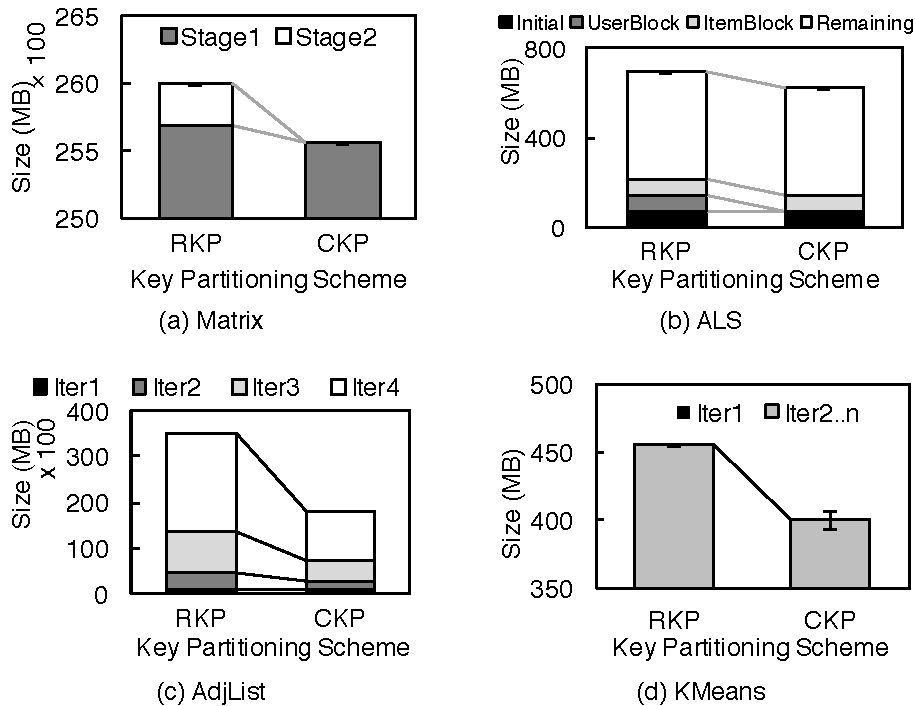
\includegraphics[width=1\columnwidth]{figure5}
\caption{The Shuffle Size and Standard Deviation of Workloads of Multiple Iterations (or Stages) in MatrixMultiplication (Matrix), MovieLensALS (ALS), MultiAdjacentList (AdjList) and KMeans Benchmarks
}
\label{fig:size}
%\vspace{-0.2in}
\end{figure}


\subsection{Shuffle Size Improvement} 
Results of the shuffle size and the workload skewness of each iteration (or stage) after applying CKP and RKP in all the benchmarks are shown in Fig.~\ref{fig:size}, respectively. 

In MatrixMultiplication, CKP totally removes the shuffle size of stage 2, and the shuffle size of stage 1 remains close to that of RKP (Fig.~\ref{fig:size}(a)). 
Note that, regardless of the key partitioning scheme, the volume of data in stage 2 is small compared to stage 1 because data have been locally merged by the distributed framework to compress data in stage 2~\cite{zaharia2012resilient}.
% Still, we will show that CKP has the advantage in minimizing the job completion time by eliminating the shuffle runtime overheads in the latter sub-sections. 

The benefit of applying CKP on iterative distributed operations 
that reduce the key dimensions can be read in Fig.~\ref{fig:size}(b).
In MovieLensALS, after applying CKP, the shuffle size for generating the user block is 0, while the shuffle size for generating the item block remains almost the same as that of RKP. 
As a result, the CKP shuffle size for generating these two block is half of that of RKP. 
Because the other iterations of the distributed operations cannot be improved by CKP, 
the overall shuffle size CKP can reduce for this application is about 11\%.

After applying CKP in MultiAdjacentList benchmark, the shuffle size of each iteration is decreased by half beginning from iteration 2 (Fig.~\ref{fig:size}(c)). 
The reason is that by binding partitions of key $(list, tail)$ 
to key $list$, only data with key $(head, list)$ need to be shuffled in each iteration, which is about 50\% of the total data volume. 

In KMeans benchmark, points are bound to centers they are grouped into in iteration 1. by partitioning the points into clusters they belong to in the first iteration, CKP decreases the overall shuffle size by 12\% (Fig.~\ref{fig:size}(d)). 
This decrease in shuffle size is contributed by avoiding the repartition of the points that are stable to their clusters,
although not all points are fixed to their clusters in every iteration. 
This shuffle size is influenced by the input dataset, initial 
centroids of clusters, and from which iteration the points are bound to the centroids.
All these factors affect the dependency probability in the key dependency.

Note that the shuffle sizes of the other iterations that do not apply CKP remains almost unchanged, which means that CKP can decrease the shuffle size of distributed iterations that have the confluence key dependency without introducing extra workloads to the other iterations. 
How CKP can decrease the overall shuffle traffic depends on how large the volumes of data are in iterations that apply key partition binding, compared to the overall data volume of the application. 
For MultiAdjacentList, the CKP can be applied to half of the operations, either appending to the head or to the tail.
While for MovieLensALS, CKP can only be applied to the operation that arrange the user-item blocks, which is a relatively small portion of the overall application. 
Still, it indicates the potential of applying CKP in the complicated iterative distributed applications. 


% \begin{figure}[!t]
% \centering
% 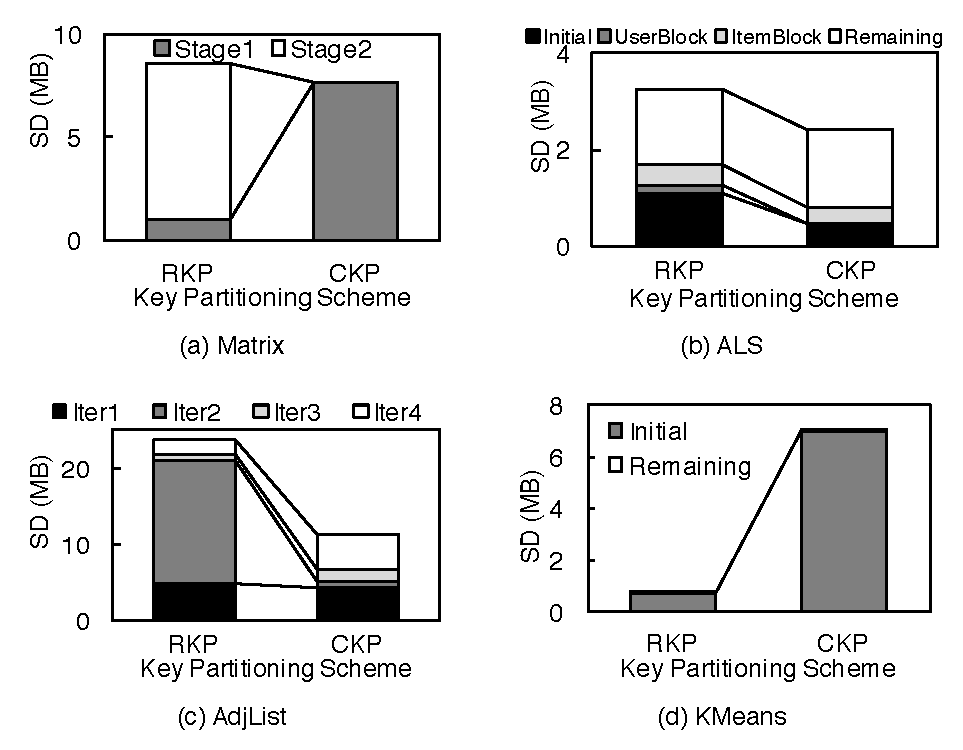
\includegraphics[width=1\columnwidth]{figure6}
% \caption{Standard Deviations (SD) of the Shuffle Sizes of the Executors of Multiple Iterations (or Stages) in MatrixMultiplication (Matrix), MovieLensALS (ALS), MultiAdjacentList (AdjList) and KMeans Benchmarks
% }
% \label{fig:SD}
% %\vspace{-0.2in}
% \end{figure}

\subsection{Workload Skew}
The workload skewness is denoted as the standard deviation bar in Fig.~\ref{fig:size}. 
As expected, the workload skewness (standard deviation of workloads) of the key partition 
binding stages of MatrixMultiplication (Fig.~\ref{fig:size}(a)), MovieLensALS (Fig.~\ref{fig:size}(b)) and MultiAdjacentList (Fig.~\ref{fig:size}(c)) are all close to 0. 
In the KMeans benchmark, the workload skewness of CKP is larger than that in RKP (Fig.~\ref{fig:size}(d)). 
The reason is that the number of points belonging to each cluster varies but the number of clusters (32) is not large enough compared to 
the computer nodes (16) to balance the workloads of the nodes. 
If the number of clusters is larger, 
the number of points bound to each cluster is smaller.
As each cluster centroid is randomly partitioned, the workload 
skewness will become smaller.
Still, the standard deviation of CKP (7 MB) is small as compared to the mean shuffle size of the executors (25 MB).


% For the stages that are either before or after the CKP-affected stages, the standard deviations remain almost the same as RKP, or as compared to the shuffle size, the difference is so tiny that can be ignored. 

\begin{figure}[!t]
\centering
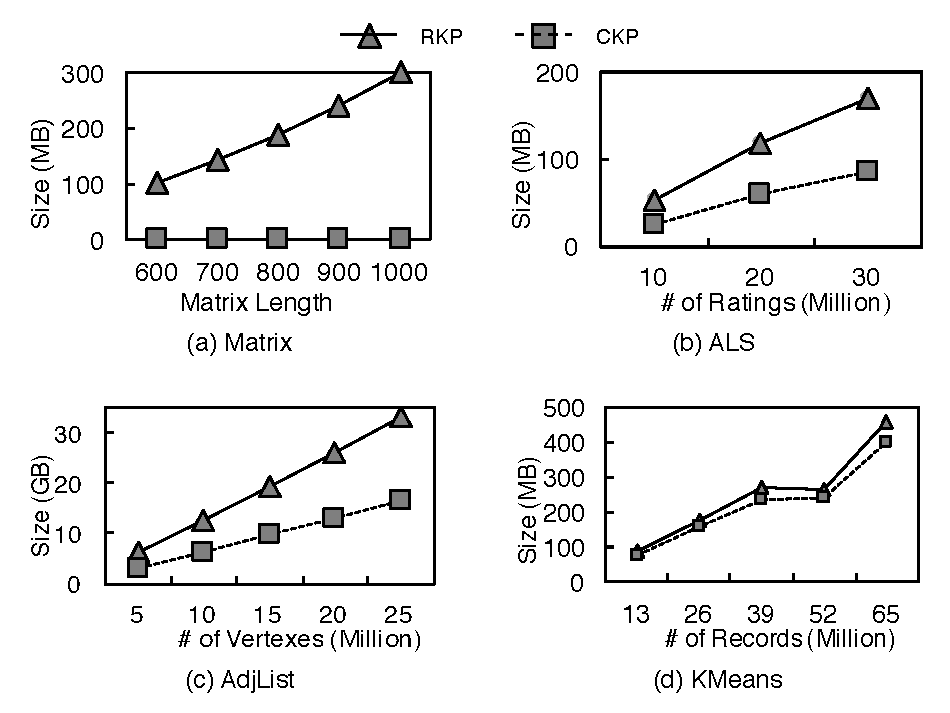
\includegraphics[width=1\columnwidth]{figure7}
\caption{Overall Shuffle Size of the Key Partition 
Binding Iterations in MatrixMultiplication (Matrix), MovieLensALS (ALS), MultiAdjacentList (AdjList) and KMeans Benchmarks with Different Input Size}
\label{fig:sizeLine}
%\vspace{-0.2in}
\end{figure}


\subsection{Scalability}
The overall shuffle sizes of iterations that apply key partition 
binding with different input sizes in various benchmarks are shown in Fig.~\ref{fig:sizeLine}. 
In MatrixMultiplication, 
the overall shuffle size of RKP increases linearly as the matrix length grows, while that of CKP is always 0. 
CKP can totally remove the shuffle size of stage 2 in MatrixMultiplication. 
In the other benchmarks, the shuffle sizes of CKP always keep in a fixed (or stable) ratio to those of RKP, e.g., 50\% in both MovieLensALS and MultiAdjacentList and around 88\% in KMeans. 
The result shows that CKP scales well with different volumes of input data. 
The CKP decreases the shuffle size greatly (about 50\%) in one iteration out of many iterations in the MovieLensALS application, and a little (about 12\%) but in every iteration the KMeans application. 



\section{Related Work}\label{section:relatedWork}
\textbf{Iterative distributed computing}: 
Some works~\cite{gunarathne2013scalable, zaharia2012resilient,bu2010haloop, ekanayake2010twister} improved distributed frameworks for iterative distributed operations by extending programming interfaces to support multiple transform and shuffle phases. 
The general idea was to cache the data of each iteration in memories instead of in disks to reduce I/O overheads.
% Spark~\cite{zaharia2012resilient} provided more kinds of operation interfaces and supported a series of transformations on input datasets in the memory by the concept of resilient distributed dataset. 
% These iterative distributed frameworks tried to minimize the I/O overhead by storing the intermediate data of each iteration in the memory, instead of in the disk like Hadoop. 
However, these works on distributed frameworks did not concern with the heavy network workload during shuffle operations. 
Inheriting the benefit of fast memory I/O rate, CKP decreases shuffle sizes and alleviate network workloads by considering the key dependency in multiple related iterations. 

\textbf{Parallel\&Distributed algorithms optimization}: Lots of work has been conducted on the optimization of parallel\&distributed machine learning algorithms~\cite{bekkerman2011scaling} and science computing~\cite{kiran2013verification, mensink2012metric}, including matrix multiplication methods~\cite{buluc2012parallel, ballard2012communication}. 
Generally, they focused on optimizing the algorithm itself by decomposing tasks to increase task parallelism or removing the synchronization boundary between I/O-intensive tasks and compute-intensive tasks. 
Sarma et al.~\cite{Sarma:2013:ULB} represented the number of data entries generated from the map input for a distributed application with a given parallelism factor as communication cost. 
To decrease the communication cost for a specific distributed application, one need redesign the logic of the program itself, operating with the proper parallelism factor. 
The term of communication cost is slightly different from the shuffle size in this paper, where the communication cost is the transfer size of data between different reduce workers (which can be on the same node), while the shuffle size is transfer size of data between different computer nodes. 
An iterative distributed application can first be designed with the minimum communication cost for each iteration, if possible, and then apply CKP to decrease the shuffle size.
% The algorithms with the minimum communication cost can further decrease the shuffle size by considering the key dependency of the datasets in multiple iterations. 
ShuffleWatcher~\cite{faraz2014shufflewatcher} scheduled the locality of map tasks and reduce tasks to decrease shuffle size for the single 
iteration of a MapReduce job, but it did not provide a solution for iterative distributed operations. 

\textbf{Logic-Aware Shuffle Partitioning}: 
Some similar works~\cite{zhou2010scope, zhang2012shuffle} also looked into the logic of programs and considered the data relation across iterations to avoid unnecessary shuffle network traffic. 
But the methods either lacked a precise model abstraction so that 
its applicable area was limited to aggregate-like operations~\cite{zhang2012shuffle}, or built a complicated model that made its usage difficult~\cite{zhou2010scope}. The Confluence key dependency model is simple in form
and makes it possible to apply CKP in a single line of code. 
The dependency probability easily predicts the effect of 
shuffle size reduction.

\textbf{Datacenter networking for shuffle}: 
In datacenters, various networking scheduling algorithms were proposed to improve the shuffle throughput for different performance goals~\cite{greenberg2009vl2,popa2012faircloud,shieh2011sharing,chowdhury2011managing}.  
CKP does not concern with the underlying network level. However, by decreasing shuffle workloads, shuffle operations applying CKP can work on these shuffle-optimized datacenter networks seamlessly and gain larger performance increase.


\textbf{Skew\&Straggler}: 
Distributed computing paradigms like MapReduce adopted the data locality principle, either to place computing tasks close to locations of the processing data in priority to avoid data migration~\cite{dean2008mapreduce, zaharia2008improving}, or to avoid an unbalanced allocation of workloads by considering compute skew problems~\cite{kwon2010skew, kwon2012skewtune}. 
They concerned with the placing of map tasks whose required input data are self-contained.
As the input data of each shuffle task are distributed across the cluster, such a task-to-data approach cannot help in shuffle tasks. 
CKP binds key partitions of different iterations based on the key dependency, which eliminates shuffle traffic of multiple iterations while not impacting the balance of workloads.
Aaron et al.~\cite{Harlap:2016:ASP} addressed the problem of stragglers in iterative machine learning. 
In the case of successive key partition binding,
as CKP randomly partitions mapped keys in every iteration 
whose next iteration does not apply key partition binding, 
the workload skewness always readjusts to balanced. 

% \textbf{DAG scheduling}: 
% Similar to other DAG task scheduling algorithms~\cite{sakellariou2004hybrid, zhao2006scheduling, spark-dagscheduler, isard2007dryad} that schedule tasks to based on the task dependency graph, Confluence optimizes the partition location based on the key dependency graph. 
% The difference is, in terms of the goal, that the DAG task scheduling algorithms tried to parallel the execution of jobs that are not depended on each other to increase parallelism, while Confluence isolates the partitions of the key-related data in multiple shuffle iterations to reduce network traffic. 


\section{Conclusion and Future Work}\label{section:conclusion}
We have presented the Confluence Key Partitioning (CKP) scheme, the first work on reducing the shuffle size of
iterative distributed operations based on the key dependency. 
The key dependency precisely captures the logic of iterative distributed operations and CKP partitions data across different iterations by using the technique of key partition binding.
CKP greatly reduces the overall shuffle size with a predictable value 
while not introducing the workload skewness side effect 
for a variety of distributed operations
in fields such as scientific computing, machine learning, data
analysis.

In the future, we will try to explore methods to automatically discover the key dependency of data among different iterations. 
A potential feasible solution is data flow tracking. 
With a set of sampled data, we can keep track of how data are flowing between nodes across different iterations, and thus find out the key dependency of these sampled data. 
The challenge is that how to expand key dependency of the sample data to the whole dataset. 
Unrepresentative sample data affect the accuracy of the dependency probability. 
Luckily, as we have discussed, CKP survives the problem inaccurate dependency probability.

% \bigskip
% \noindent
% {\bf Acknowledgement}
% This work is supported in part by a Hong Kong RGC CRF grant
% (C7036-15G).

%% use section* for acknowledgment
\ifCLASSOPTIONcompsoc
 % The Computer Society usually uses the plural form
 \section*{Acknowledgments}
\else
 % regular IEEE prefers the singular form
 \section*{Acknowledgment}
\fi
This work is supported in part by a Hong Kong RGC CRF grant
(C7036-15G).


% An example of a floating figure using the graphicx package.
% Note that \label must occur AFTER (or within) \caption.
% For figures, \caption should occur after the \includegraphics.
% Note that IEEEtran v1.7 and later has special internal code that
% is designed to preserve the operation of \label within \caption
% even when the captionsoff option is in effect. However, because
% of issues like this, it may be the safest practice to put all your
% \label just after \caption rather than within \caption{}.
%
% Reminder: the "draftcls" or "draftclsnofoot", not "draft", class
% option should be used if it is desired that the figures are to be
% displayed while in draft mode.
%
%\begin{figure}[!t]
%\centering
%\includegraphics[width=2.5in]{myfigure}
% where an .eps filename suffix will be assumed under latex, 
% and a .pdf suffix will be assumed for pdflatex; or what has been declared
% via \DeclareGraphicsExtensions.
%\caption{Simulation results for the network.}
%\label{fig_sim}
%\end{figure}

% Note that IEEE typically puts floats only at the top, even when this
% results in a large percentage of a column being occupied by floats.
% However, the Computer Society has been known to put floats at the bottom.


% An example of a double column floating figure using two subfigures.
% (The subfig.sty package must be loaded for this to work.)
% The subfigure \label commands are set within each subfloat command,
% and the \label for the overall figure must come after \caption.
% \hfil is used as a separator to get equal spacing.
% Watch out that the combined width of all the subfigures on a 
% line do not exceed the text width or a line break will occur.
%
%\begin{figure*}[!t]
%\centering
%\subfloat[Case I]{\includegraphics[width=2.5in]{box}%
%\label{fig_first_case}}
%\hfil
%\subfloat[Case II]{\includegraphics[width=2.5in]{box}%
%\label{fig_second_case}}
%\caption{Simulation results for the network.}
%\label{fig_sim}
%\end{figure*}
%
% Note that often IEEE papers with subfigures do not employ subfigure
% captions (using the optional argument to \subfloat[]), but instead will
% reference/describe all of them (a), (b), etc., within the main caption.
% Be aware that for subfig.sty to generate the (a), (b), etc., subfigure
% labels, the optional argument to \subfloat must be present. If a
% subcaption is not desired, just leave its contents blank,
% e.g., \subfloat[].


% An example of a floating table. Note that, for IEEE style tables, the
% \caption command should come BEFORE the table and, given that table
% captions serve much like titles, are usually capitalized except for words
% such as a, an, and, as, at, but, by, for, in, nor, of, on, or, the, to
% and up, which are usually not capitalized unless they are the first or
% last word of the caption. Table text will default to \footnotesize as
% IEEE normally uses this smaller font for tables.
% The \label must come after \caption as always.
%
%\begin{table}[!t]
%% increase table row spacing, adjust to taste
%\renewcommand{\arraystretch}{1.3}
% if using array.sty, it might be a good idea to tweak the value of
% \extrarowheight as needed to properly center the text within the cells
%\caption{An Example of a Table}
%\label{table_example}
%\centering
%% Some packages, such as MDW tools, offer better commands for making tables
%% than the plain LaTeX2e tabular which is used here.
%\begin{tabular}{|c||c|}
%\hline
%One & Two\\
%\hline
%Three & Four\\
%\hline
%\end{tabular}
%\end{table}


% Note that the IEEE does not put floats in the very first column
% - or typically anywhere on the first page for that matter. Also,
% in-text middle ("here") positioning is typically not used, but it
% is allowed and encouraged for Computer Society conferences (but
% not Computer Society journals). Most IEEE journals/conferences use
% top floats exclusively. 
% Note that, LaTeX2e, unlike IEEE journals/conferences, places
% footnotes above bottom floats. This can be corrected via the
% \fnbelowfloat command of the stfloats package.



% if have a single appendix:
%\appendix[Proof of the Zonklar Equations]
% or
%\appendix  % for no appendix heading
% do not use \section anymore after \appendix, only \section*
% is possibly needed

% use appendices with more than one appendix
% then use \section to start each appendix
% you must declare a \section before using any
% \subsection or using \label (\appendices by itself
% starts a section numbered zero.)
%


%\appendices
%\section{Proof of the First Zonklar Equation}
%Appendix one text goes here.
%
%% you can choose not to have a title for an appendix
%% if you want by leaving the argument blank
%\section{}
%Appendix two text goes here.
%
%


%
%
%The authors would like to thank...


% Can use something like this to put references on a page
% by themselves when using endfloat and the captionsoff option.
%\ifCLASSOPTIONcaptionsoff
%  \newpage
%\fi



% trigger a \newpage just before the given reference
% number - used to balance the columns on the last page
% adjust value as needed - may need to be readjusted if
% the document is modified later
%\IEEEtriggeratref{22}
% The "triggered" command can be changed if desired:
%\IEEEtriggercmd{\enlargethispage{-5in}}

% references section

% can use a bibliography generated by BibTeX as a .bbl file
% BibTeX documentation can be easily obtained at:
% http://www.ctan.org/tex-archive/biblio/bibtex/contrib/doc/
% The IEEEtran BibTeX style support page is at:
% http://www.michaelshell.org/tex/ieeetran/bibtex/
% \bibliographystyle{IEEEtran}
% % argument is your BibTeX string definitions and bibliography database(s)
% \bibliography{IEEELonger}
%
% <OR> manually copy in the resultant .bbl file
% set second argument of \begin to the number of references
% (used to reserve space for the reference number labels box)
%\begin{thebibliography}{1}
% Generated by IEEEtran.bst, version: 1.13 (2008/09/30)
\begin{thebibliography}{44}
\providecommand{\url}[1]{#1}
\csname url@samestyle\endcsname
\providecommand{\newblock}{\relax}
\providecommand{\bibinfo}[2]{#2}
\providecommand{\BIBentrySTDinterwordspacing}{\spaceskip=0pt\relax}
\providecommand{\BIBentryALTinterwordstretchfactor}{4}
\providecommand{\BIBentryALTinterwordspacing}{\spaceskip=\fontdimen2\font plus
\BIBentryALTinterwordstretchfactor\fontdimen3\font minus
  \fontdimen4\font\relax}
\providecommand{\BIBforeignlanguage}[2]{{%
\expandafter\ifx\csname l@#1\endcsname\relax
\typeout{** WARNING: IEEEtran.bst: No hyphenation pattern has been}%
\typeout{** loaded for the language `#1'. Using the pattern for}%
\typeout{** the default language instead.}%
\else
\language=\csname l@#1\endcsname
\fi
#2}}
\providecommand{\BIBdecl}{\relax}
\BIBdecl

\bibitem{Malewicz:2010:PSL}
G.~Malewicz et al., ``Pregel: A system for large-scale graph processing,'' in
  \emph{Proceedings of the ACM SIGMOD International Conference on Management of
  Data}, New York, NY, USA, 2010, pp. 135--146.

\bibitem{Ousterhout2015MSP}
K.~Ousterhout et al., ``Making Sense of Performance in Data Analytics Frameworks,'' \emph{NSDI}, vol.~15, pp.~293-307, 2015.

\bibitem{Lu:2014:LDG}
Y.~Lu et al., ``Large-scale distributed graph computing
  systems: An experimental evaluation,'' \emph{Proceedings of the VLDB
  Endowment}, vol.~8, no.~3, pp. 281--292, 2014.

\bibitem{thusoo2009hive}
A.~Thusoo et al., ``Hive: A warehousing solution over a map-reduce
  framework,'' \emph{Proceeding of VLDB Endowment}, vol.~2, no.~2, pp.
  1626--1629, 2009.

\bibitem{Yu:2008:DSG}
Y.~Yu et al., ``Dryadlinq: A system for general-purpose distributed
  data-parallel computing using a high-level language,'' in \emph{Proceedings
  of the 8th USENIX Symposium on Operating Systems Design and Implementation},
  2008, pp. 1--14.

\bibitem{Armbrust:2015:SSR}
M.~Armbrust et al., ``Spark sql: Relational
  data processing in spark,'' in \emph{Proceedings of the 2015 ACM SIGMOD
  International Conference on Management of Data}, New York, NY, USA, 2015, pp. 1383--1394.

\bibitem{low2012distributed}
Y.~Low et al.,
  ``Distributed graphlab: A framework for machine learning and data mining in
  the cloud,'' \emph{Proceedings of the VLDB Endowment}, vol.~5, no.~8, pp.
  716--727, 2012.

\bibitem{kraska2013mlbase}
T.~Kraska et al., ``Mlbase: A distributed machine-learning system,'' in
  \emph{Conference on Innovative Data Systems Research (CIDR)}, vol.~1, 2013,
  pp. 2--1.

\bibitem{vavilapalli2013apache}
V.~K. Vavilapalli et al., ``Apache hadoop yarn: Yet another
  resource negotiator,'' in \emph{Proceedings of the 4th ACM Annual Symposium
  on Cloud Computing}, New York, NY, USA, 2013, pp. 5:1--5:16.

% \bibitem{hindman2011mesos}
% B.~Hindman et al., ``Mesos: A platform for fine-grained resource
%   sharing in the data center.'' in \emph{Proceedings of the 8th USENIX
%   Symposium on Networked Systems Design and Implementation}, vol.~11, 2011, pp.
%   22--22.

\bibitem{isard2007dryad}
M.~Isard et al., ``Dryad: Distributed
  data-parallel programs from sequential building blocks,'' in
  \emph{Proceedings of the 2nd ACM SIGOPS/EuroSys European Conference on
  Computer Systems}, New York, NY, USA, 2007, pp. 59--72.

\bibitem{white2012hadoop}
T.~White, ``Hadoop: The definitive guide'', \emph{O'Reilly Media Inc.}, 2012.

\bibitem{dean2008mapreduce}
J.~Dean and S.~Ghemawat, ``Mapreduce: Simplified data processing on large
  clusters,'' \emph{Communications of the ACM}, vol.~51, no.~1, pp. 107--113,
  2008.

\bibitem{shvachko2010hadoop}
K.~Shvachko et al., ``The hadoop distributed file
  system,'' in \emph{Proceedings of the IEEE 26th Symposium on Mass Storage
  Systems and Technologies}, 2010,
  pp. 1--10.

\bibitem{chen2011case}
Y.~Chen et al., ``The case for evaluating
  mapreduce performance using workload suites,'' in \emph{IEEE 19th
  International Symposium on Modeling, Analysis \& Simulation of Computer and
  Telecommunication Systems}, 2011, pp. 390--399.

\bibitem{chowdhury2011managing}
M.~Chowdhury et al., ``Managing data
  transfers in computer clusters with orchestra,'' in \emph{Proceedings of the
  ACM SIGCOMM Conference}, New York, NY,
  USA, 2011, pp. 98--109.

\bibitem{al2010hedera}
M.~Al-Fares et al., ``Hedera:
  Dynamic flow scheduling for data center networks.'' in \emph{Proceedings of
  the 7th USENIX conference on Networked Systems Design and Implementation},
  vol.~10, 2010, pp. 19--19.

\bibitem{bu2010haloop}
Y.~Bu et al., ``Haloop: efficient iterative
  data processing on large clusters,'' \emph{Proceedings of the VLDB
  Endowment}, vol.~3, no. 1-2, pp. 285--296, 2010.

\bibitem{zaharia2012resilient}
M.~Zaharia et al., ``Resilient distributed datasets: A fault-tolerant
  abstraction for in-memory cluster computing,'' in \emph{Proceedings of the
  9th USENIX conference on Networked Systems Design and Implementation}, 2012,
  pp. 2--2.

\bibitem{ekanayake2010twister}
J.~Ekanayake et al.,
  ``Twister: a runtime for iterative mapreduce,'' in \emph{Proceedings of the
  19th ACM International Symposium on High Performance Distributed Computing},
  2010, pp. 810--818.

\bibitem{sakellariou2004hybrid}
R.~Sakellariou and H.~Zhao, ``A hybrid heuristic for dag scheduling on
  heterogeneous systems,'' in \emph{Proceedings of 18th IEEE International
  Parallel and Distributed Processing Symposium}, 2004, pp. 111--.

\bibitem{zhao2006scheduling}
H.~Zhao and R.~Sakellariou, ``Scheduling multiple dags onto heterogeneous
  systems,'' in \emph{Proceedings of 20th IEEE International Parallel and
  Distributed Processing Symposium}, 2006, pp. 14--.

\bibitem{movielensals}
\BIBentryALTinterwordspacing
``Movielensals spark submit 2014.'' [Online]. Available:
  \url{https://databricks-training.s3.amazonaws.com/movie-recommendation-with-mllib.html}
\BIBentrySTDinterwordspacing

\bibitem{multiAdjList}
\BIBentryALTinterwordspacing
``Multiadjacentlist benchmark.'' [Online]. Available:
  \url{https://github.com/liangfengsid/MultiAdjacentList}
\BIBentrySTDinterwordspacing

\bibitem{kmeans}
\BIBentryALTinterwordspacing
``Spark kmeans benchmark.'' [Online]. Available:
  \url{http://spark.apache.org/docs/latest/mllib-clustering.html}
\BIBentrySTDinterwordspacing

\bibitem{gideon}
\BIBentryALTinterwordspacing
``Hku gideon-ii cluster.'' [Online]. Available:
  \url{http://i.cs.hku.hk/\%7Eclwang/Gideon-II/}
\BIBentrySTDinterwordspacing

\bibitem{google2012spanner}
J.C. Corbett et al., ``Spanner: Google’s globally distributed database,'' 
\emph{Proceedings of the 10th USENIX conference on Operating Systems Design and Implementation}, pp. 251-264, 2012.

\bibitem{zhou2010scope}
J.~Zhou et al., ``Incorporating partitioning and parallel plans into the SCOPE optimizer,'' \emph{IEEE 26th International Conference on Data Engineering}, pp. 1060-1071, 2010.

\bibitem{zhang2012shuffle}
J.~Zhang et al., ``Optimizing Data Shuffling in Data-Parallel Computation by Understanding User-Defined Functions,'' \emph{NSDI}, vol.~12, pp.~22-22, 2012.

\bibitem{gunarathne2013scalable}
T.~Gunarathne et al., ``Scalable parallel computing on
  clouds using twister4azure iterative mapreduce,'' \emph{Future Generation
  Computer Systems}, vol.~29, no.~4, pp. 1035-1048, 2013.

\bibitem{bekkerman2011scaling}
R.~Bekkerman, M.~Bilenko, and J.~Langford, \emph{Scaling up machine learning:
  Parallel and distributed approaches}.\hskip 1em plus 0.5em minus 0.4em\relax
  Cambridge University Press, 2011.

\bibitem{kiran2013verification}
M.~Kiran, A.~Kumar, and B.~Prathap, ``Verification and validation of parallel
  support vector machine algorithm based on mapreduce program model on hadoop
  cluster,'' in \emph{IEEE International Conference on Advanced Computing and
  Communication Systems}, 2013, pp. 1--6.

\bibitem{mensink2012metric}
T.~Mensink et al., ``Metric learning for
  large scale image classification: Generalizing to new classes at near-zero
  cost,'' in \emph{Computer Vision--ECCV 2012}.\hskip 1em plus 0.5em minus
  0.4em\relax Springer, 2012, pp. 488--501.

\bibitem{buluc2012parallel}
A.~Buluc and J.~R. Gilbert, ``Parallel sparse matrix-matrix multiplication and
  indexing: Implementation and experiments,'' \emph{SIAM Journal on Scientific
  Computing}, vol.~34, no.~4, pp. C170--C191, 2012.

\bibitem{ballard2012communication}
G.~Ballard et al.,
  ``Communication-optimal parallel algorithm for strassen's matrix
  multiplication,'' in \emph{Proceedings of the 24th annual ACM Symposium on
  Parallelism in Algorithms and Architectures}, 2012, pp. 193--204.

\bibitem{Sarma:2013:ULB}
A.~D. Sarma et al., ``Upper and lower
  bounds on the cost of a map-reduce computation,'' \emph{Proceedings of the
  VLDB Endowment}, vol.~6, no.~4, pp. 277--288, 2013.

\bibitem{faraz2014shufflewatcher}
F.~Ahmad et al.,
  ``Shufflewatcher: Shuffle-aware scheduling in multi-tenant mapreduce
  clusters,'' in \emph{2014 USENIX Annual Technical Conference}, Philadelphia, PA, Jun. 2014, pp. 1--13.

\bibitem{greenberg2009vl2}
A.~Greenberg et al., ``Vl2: a scalable and flexible data center
  network,'' in \emph{Communication of the ACM}, vol.~54, no.~3, 2011, pp.
  95--104.

\bibitem{popa2012faircloud}
L.~Popa et al.,
  ``Faircloud: sharing the network in cloud computing,'' in \emph{Proceedings
  of the ACM SIGCOMM conference on Applications, technologies, architectures,
  and protocols for computer communication}, 2012, pp. 187--198.

\bibitem{shieh2011sharing}
A.~Shieh et al., ``Sharing the data
  center network,'' in \emph{Proceedings of the 8th USENIX Symposium on
  Networked Systems Design and Implementation}, 2011, pp. 309--322.

\bibitem{zaharia2008improving}
M.~Zaharia et al., ``Improving
  mapreduce performance in heterogeneous environments,'' in \emph{Proceedings
  of the 8th USENIX Symposium on Operating Systems Design and Implementation},
  2008, pp. 29--42.

\bibitem{kwon2010skew}
Y.~Kwon et al., ``Skew-resistant parallel
  processing of feature-extracting scientific user-defined functions,'' in
  \emph{Proceedings of the 1st ACM Symposium on Cloud Computing}, 2010, pp. 75--86.

\bibitem{kwon2012skewtune}
Y.~Kwon et al., ``Skewtune: mitigating skew in mapreduce applications,'' in
  \emph{Proceedings of the ACM SIGMOD International Conference on Management of
  Data}, 2012, pp. 25--36.

\bibitem{Harlap:2016:ASP}
A.~Harlap et al., ``Addressing the straggler problem for iterative convergent
  parallel ml,'' in \emph{Proceedings of the Seventh ACM Symposium on Cloud
  Computing}, New York, NY, USA, 2016, pp. 98--111.

\bibitem{spark-dagscheduler}
\BIBentryALTinterwordspacing
Spark job scheduling: Dagscheduler. [Online]. Available:
  \url{https://spark.apache.org/docs/1.4.0/job-scheduling.html}
\BIBentrySTDinterwordspacing

\end{thebibliography}

%
%\bibitem{IEEEhowto:kopka}
%H.~Kopka and P.~W. Daly, \emph{A Guide to \LaTeX}, 3rd~ed.\hskip 1em plus
%  0.5em minus 0.4em\relax Harlow, England: Addison-Wesley, 1999.
%
%\end{thebibliography}

% biography section
% 
% If you have an EPS/PDF photo (graphicx package needed) extra braces are
% needed around the contents of the optional argument to biography to prevent
% the LaTeX parser from getting confused when it sees the complicated
% \includegraphics command within an optional argument. (You could create
% your own custom macro containing the \includegraphics command to make things
% simpler here.)
%\begin{IEEEbiography}[{\includegraphics[width=1in,height=1.25in,clip,keepaspectratio]{mshell}}]{Michael Shell}
% or if you just want to reserve a space for a photo:
\newpage

\vspace{-.5in}
\begin{IEEEbiography}[{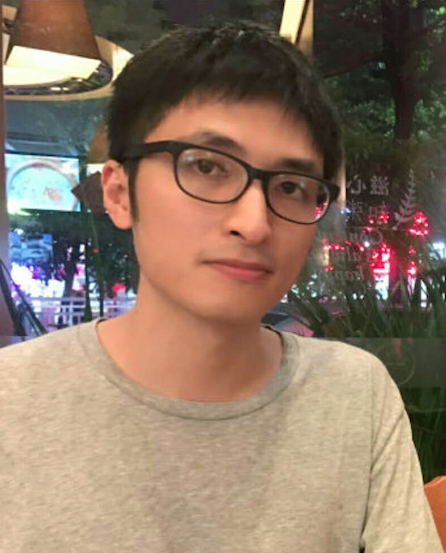
\includegraphics[width=1in,height=1.25in,clip,keepaspectratio]{author1}}]{Feng Liang}
received the BS degree in software engineering from Nanjing University in 2012, and the PhD degree in computer science from The University of Hong Kong in 2017. His research interests are mainly on distributed file systems, distributed computing, machine learning, and formal methods for distributed systems. He is recently undertaking the research project on distributed deep learning.
[homepage] i.cs.hku.hk/\%7Efliang
\end{IEEEbiography}

\vspace{-1.5in}
\begin{IEEEbiography}[{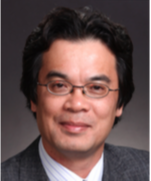
\includegraphics[width=1in,height=1.25in,clip,keepaspectratio]{author2}}]{Francis C.M. Lau}
received his PhD in computer science from the University of Waterloo in 1986. He has been a faculty member of the Department of Computer Science, The University of Hong Kong since 1987, where he served as the department chair from 2000 to 2005. He is now Associate Dean of Faculty of Engineering, the University of Hong Kong. He was a honorary chair professor in the Institute of Theoretical Computer Science of Tsinghua University from 2007 to 2010. His research interests include
computer systems and networking, algorithms, HCI, and application of IT to arts. He is the editor-in-chief of the Journal of Interconnection Networks.
[homepage] i.cs.hku.hk/\%7Efcmlau
\end{IEEEbiography}

\vspace{-1.5in}
\begin{IEEEbiography}[{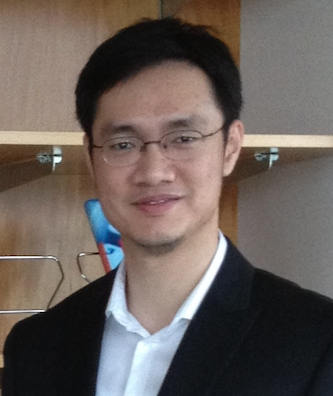
\includegraphics[width=1in,height=1.25in,clip,keepaspectratio]{author3}}]{Heming Cui}
is an assistant professor in Computer Science of HKU. His research interests are in operating systems, programming languages, distributed systems, and cloud computing, with a particular focus on building software infrastructures and tools to improve reliability and security of real-world software. 
[homepage] i.cs.hku.hk/\%7Eheming
\end{IEEEbiography}

\vspace{-1.5in}
\begin{IEEEbiography}[{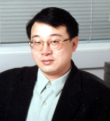
\includegraphics[width=1in,height=1.25in,clip,keepaspectratio]{author4}}]{Cho-Li Wang}
is currently a Professor in the Department of Computer Science at The
University of Hong Kong. He graduated with a B.S. degree in Computer Science and
Information Engineering from National Taiwan University in 1985 and a Ph.D.
degree in Computer Engineering from University of Southern California in 1995. Prof.
Wang’s research is broadly in the areas of parallel architecture, software systems for
Cluster computing, and virtualization techniques for Cloud computing. His recent
research projects involve the development of parallel software systems for
multicore/GPU computing and multi-kernel operating systems for future manycore
processor. Prof. Wang has published more than 150 papers in various peer reviewed
journals and conference proceedings. He is/was on the editorial boards of several scholarly
journals, including IEEE Transactions on Cloud Computing (2013-), IEEE
Transactions on Computers (2006-2010).
[homepage] i.cs.hku.hk/\%7Eclwang
\end{IEEEbiography}

% insert where needed to balance the two columns on the last page with
% biographies
%\newpage



% You can push biographies down or up by placing
% a \vfill before or after them. The appropriate
% use of \vfill depends on what kind of text is
% on the last page and whether or not the columns
% are being equalized.

%\vfill

% Can be used to pull up biographies so that the bottom of the last one
% is flush with the other column.
%\enlargethispage{-5in}



% that's all folks
\end{document}


